\chapter{The Deep Underground Neutrino Experiment}
\label{chapter:dune}

\begin{chapquote}{Frank Herbert, \textit{Dune}}
	Deep in the human unconscious is a pervasive need for a logical universe that makes sense. But the real universe is always one step beyond logic.
\end{chapquote}

%\noindent
The Deep Underground Neutrino Experiment (DUNE) is a next generation long-baseline neutrino experiment \cite{DUNE2020TDR1}.  It will aim to address several questions in neutrino physics, study neutrinos from astrophysical sources and search for beyond the standard model physics.

This Chapter reviews the main goals of the DUNE experiment, the design of the far detector modules and their data acquisition (DAQ) system, and the role that the near detector plays in the physics program of DUNE.

\section{Overview}

The main physics goals of DUNE are:
\begin{itemize}
	\item measure the neutrino mass hierarchy, the amount of CP violation in the leptonic sector and the $\theta_{23}$ octant,
	\item detect rare low energy neutrino events, like neutrinos from supernova bursts, and
	\item search for proton decay and other beyond the standard model phenomena.
\end{itemize}

The design of DUNE has been tailored with these goals in mind. It will consist of two neutrino detectors. A near detector (ND) complex will be placed at Fermilab, $574~\mathrm{m}$ downstream of the neutrino production point, whereas a larger far detector (FD) will be built in the Sandford Underground Research Facility (SURF), South Dakota, approximately $1300~\mathrm{km}$ away. Figure \ref{fig:dune} shows a simplified view of the various components of DUNE (not to scale).

\begin{figure}[t]
	\centering
	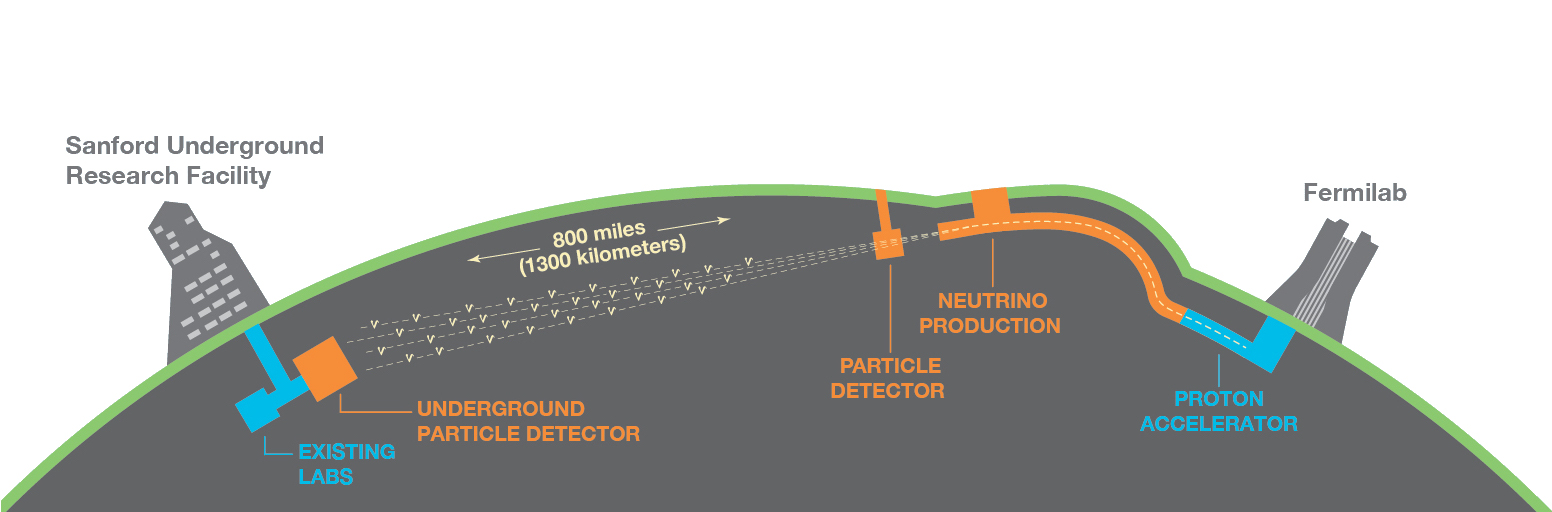
\includegraphics[width=0.9\linewidth]{Images/DUNE/FD/dune}
	\caption[Schematic diagram of the DUNE experiment and the LBNF beamline.]{Schematic diagram of the DUNE experiment and the LBNF beamline \cite{DUNE2020TDR1}.}
	\label{fig:dune}
\end{figure}

The beam neutrinos will be provided by the Long-Baseline Neutrino Facility (LBNF) beamline, the multi-megawatt wide-band neutrino beam planned for Fermilab. It will produce neutrinos travelling in the direction of SURF, with the capability to switch between neutrino and antineutrino mode.

Before arriving to the FD, the neutrino beam meets the ND complex, which serves as the experiment's control. The design of the DUNE ND is mainly driven by the needs of the oscillation physics program, as its main role is to measure the unoscillated neutrino energy spectra. From these we can predict the unoscillated spectra at the FD, which can be compared to the spectra measured at the FD to extract the oscillation parameters. Additionally, the ND has a physics programme of its own, including cross section measurements and BSM physics searches.

The technology chosen for the FD modules of DUNE is the liquid Argon time projection chamber (LArTPC). Its four modules will record neutrino interactions from the accelerator-produced beam arriving at predictable times. As it also aims at recording rare and low energy events, like supernovae and solar neutrinos, the FD requires trigger schemes which can deal with both kinds of physics, and also maximum uptime.

\begin{table}[]
	\caption[Summary of the two-phased plan for DUNE.]{Summary of the two-phased plan for DUNE. Adapted from Ref. \cite{DUNE2022Snowmass}.}
	\centering
	\begin{tabular}{c|C{3.0cm}|C{3.0cm}|c}
	Parameter  & Phase I                     & Phase II		& Benefit \\[1mm] \hline
	\rule{0pt}{1.1\normalbaselineskip}FD mass    & $20 \ \mathrm{kt}$ fiducial & $40 \ \mathrm{kt}$ fiducial & FD statistics\\[1mm]
	Beam power & up to $1.2 \ \mathrm{MW}$   & $2.4 \ \mathrm{MW}$      & FD statistics  \\[1mm]
	ND config.  & ND-LAr, TMS, SAND           & ND-LAr, ND-GAr, SAND & Systematic constraints
	\end{tabular}
	\label{tab:dune_phases}
\end{table}

DUNE is planned to be built using a staged approach consisting on two phases, which are summarised in Tab. \ref{tab:dune_phases}. Phase I consists of a FD with $50\%$ of the total fiducial mass, a reduced version of the ND complex and a $1.2~\mathrm{MW}$ proton beam. It will be sufficient to achieve some early physics goals, like the determination of the neutrino mass ordering. For its Phase II, DUNE will feature the full four FD modules, a more capable ND and a $2.4~\mathrm{MW}$ proton beam. The physics milestones for the two phases are given in Tab. \ref{tab:dune_phases_physics}, in a staging scenario which assumes that Phase II is completed after 6 years of operation.

A summary of the DUNE science program can be found in the DUNE FD Technical Design Report (TDR) Volume I \cite{DUNE2020TDR1}. For a detailed discussion on the two-phased approach the reader is referred to the DUNE Snowmass 2021 report \cite{DUNE2022Snowmass}.

\section{Physics goals of DUNE}

\begin{table}[]
	\caption[Exposure and time required to achieve the different physics milestones of the two phases.]{Exposure and time required to achieve the different physics milestones of the two phases. The predictions assume a Phase II staging scenario where FD modules 3 and 4 are deployed in years 4 and 6 and both the beam and ND are upgraded after 6 years. Adapted from Ref. \cite{DUNE2022Snowmass}.}
	\centering
	\begin{tabular}{c|c|C{3.0cm}|C{2.0cm}}
	Stage    & Physics milestone                                          & Exposure (kt-MW-years) & Years (staged) \\[3mm] \hline
	\rule{0pt}{1.1\normalbaselineskip}Phase I  & $5\sigma$ MO ($\delta_{CP} = -\pi/2$)                      & 16                     & 1-2            \\[1mm]
			 & $5\sigma$ MO ($100\%$ of the $\delta_{CP}$ values)         & 66                     & 3-5            \\[1mm]
			 & $3\sigma$ CPV ($\delta_{CP} = -\pi/2$)                     & 100                    & 4-6            \\[1mm] \hline
			 \rule{0pt}{1.1\normalbaselineskip}Phase II & $5\sigma$ CPV ($\delta_{CP} = -\pi/2$)                     & 334                    & 7-8            \\[1mm]
			 & $\delta_{CP}$ resolution of $10$ degrees ($\delta_{CP}=0$) & 400                    & 8-9            \\[1mm]
			 & $5\sigma$ CPV ($50\%$ of the $\delta_{CP}$ values)         & 646                    & 11             \\[1mm]
			 & $3\sigma$ CPV ($75\%$ of the $\delta_{CP}$ values)         & 936                    & 14             \\[1mm]
			 & $\mathrm{sin}^{2}(2\theta_{13})$ resolution of $0.004$       & 1079                   & 16            
	\end{tabular}
	\label{tab:dune_phases_physics}
\end{table}

As noted in the literature (see for instance Ref. \cite{deSalas2020} for a review), the parameter space of the neutrino oscillation phenomena within the three-flavour picture is quite constrained by current experimental data. However, there are still crucial open questions, like the mass ordering, the value of $\delta_{CP}$ or the $\theta_{23}$ octant. One of the main goals of DUNE is to determine precisely the values of these parameters \cite{DUNE2020TDR2}.

To address these questions DUNE can look to the subdominant oscillation channel $\nu_{\mu} \rightarrow \nu_{e}$ ($\bar{\nu}_{\mu} \rightarrow \bar{\nu}_{e}$) and study the energy dependence of the $\nu_{e}$ ($\bar{\nu}_{e}$) appearance probability. When we focus on the antineutrino channel $\bar{\nu}_{\mu} \rightarrow \bar{\nu}_{e}$ there is a change in the sign of $\delta_{CP}$, thus introducing CP-violation. Moreover, due to the fact that there are no positrons in the composition of Earth, there is a sign difference for the matter effect contribution when looking to the antineutrino channel. This asymmetry is proportional to the baseline length $L$ and is sensitive to the sign of $\Delta m^{2}_{31}$, and thus to the neutrino mass ordering.

Another of the main physics goals of DUNE is the search for baryon-number violating processes. Specifically, it will try to answer the question of whether protons are stable or not. There is no symmetry argument that forbids protons from decaying, but its apparent stability seems to suggest that baryon number is conserved \cite{Super-Kamiokande2009}. However, proton decay is a usual feature of grand-unified theories, where electromagnetic, weak and strong interactions are unified above a certain energy scale \cite{Raby2006}.

As the energy deposition scale for this kind of searches is nearly the same as the one for long-baseline neutrino oscillations, DUNE will be able to look for them. It has several advantages over other experiments, such as excellent imaging and particle identification, which can be translated to lower backgrounds.

The last of the main objectives of DUNE is the detection of neutrinos originated in supernovae explosions, what is called a supernova neutrino burst (SNB). These neutrinos carry with them information about the core-collapse process, from the progenitor to the explosion and the remnant; but also may have information about new exotic physics. So far, the only neutrino events ever recorded from such a process were a few dozens of $\bar{\nu}_{e}$ events from the 1987A supernova located in the Magellanic Cloud, $50~\mathrm{kpc}$ away from Earth \cite{Kamiokande-II1987, Bionta1987}.

DUNE aims to collect SNB events. Although these are quite rare, as the expected supernovae explosion events are about one every few decades for our galaxy and Andromeda, the long lifetime of the experiment (around a few decades as well) makes it reasonable to expect some. Nowadays the main sensitivity to SNB of most experiments is to the $\bar{\nu}_{e}$ through inverse beta decay. One of the advantages of DUNE is its expected sensitivity to $\nu_{e}$, since the dominant channel will be $\nu_{e}$ CC scattering.

Moreover, due to the stringent requirements that the main physics goals set for DUNE, it will allow also to perform searches for all kind of BSM physics. Among others, DUNE will be able to look for: active-sterile neutrino mixing, non-unitarity of the PMNS matrix, non-standard interactions, Lorentz and CPT violations, neutrino trident production, light-mass DM, boosted DM and heavy neutral leptons. The reader is referred to the DUNE FD TDR Volume II \cite{DUNE2020TDR2} for a full discussion of the physics scope of DUNE.

\begin{figure}[t]
	\centering
	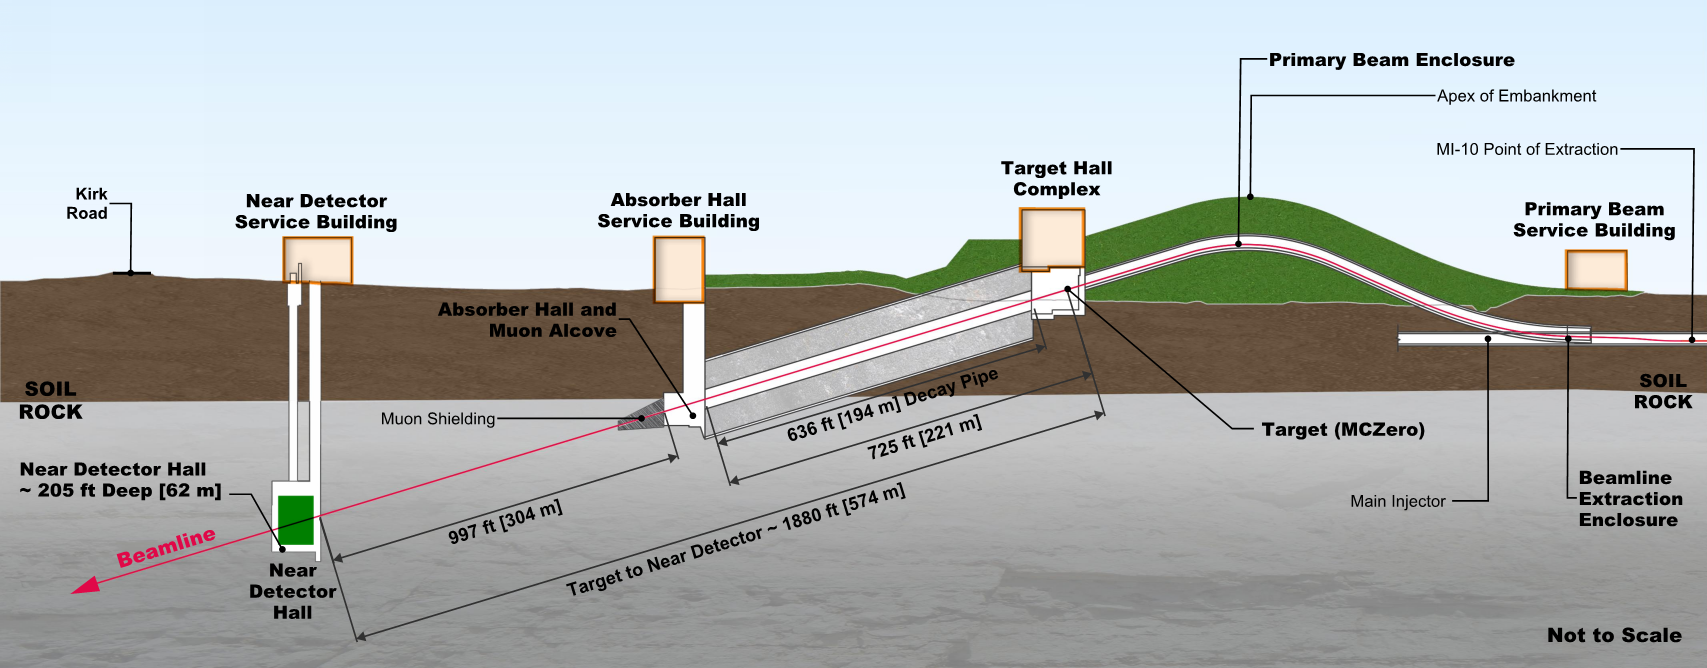
\includegraphics[width=0.95\linewidth]{Images/DUNE/LBNF/beamline-sideview}
	\caption[Schematic longitudinal section of the LBNF beamline at Fermilab.]{Schematic longitudinal section of the LBNF beamline at Fermilab (not to scale). Figure taken from Ref. \cite{DUNE2016CDR3}.}
	\label{fig:lbnf_beamline}
\end{figure}

\section{LBNF beamline}

The LBNF project is responsible for producing the neutrino beam for the DUNE detectors. A detailed discussion of the LBNF program can be found in the DUNE/LBNF CDR Volume III \cite{DUNE2016CDR3}.

A schematic diagram of the longitudinal section of the LBNF beamline is shown in Fig. \ref{fig:lbnf_beamline}. First, a beam of $60-120~\mathrm{GeV}$ protons is extracted from the Fermilab Main Injector. This beam is aimed towards the target area, where it collides with a cylindrical graphite target to produce pions and kaons.

The diffuse, secondary beam of particles is focused by a pair of magnetic horns. These select the positively charged particles when operated in Forward Horn Current (FHC) mode, or the negatively charged ones when the current is reversed, also known as Reverse Horn Current (RHC) mode. The focused secondary beam then enters a $194~\mathrm{m}$ decay pipe where the pions and kaons will predominantly produce $\mu^{+}\nu_{\mu}$ pairs when in FHC mode (or $\mu^{-}\bar{\nu}_{\mu}$ in RHC mode).

At the end of the decay pipe a hadron absorber removes the undecayed hadrons and muons from the beam, which reduces the $\nu_{e}$ ($\bar{\nu}_{e}$) and $\bar{\nu}_{\mu}$ ($\nu_{\mu}$) contamination  coming from the $\mu^{+}$ ($\mu^{-}$) decays. The resulting neutrino flux at the FD is shown in Fig. \ref{fig:dune_fd_flux}, both for FHC (left) and RHC (right) modes. These predictions show the intrinsic $\overset{\brabarb}{\nu}_{e}$ contamination and wrong sign component from wrong sign and neutral meson decays, as well as muons decaying before reaching the absorber.

\begin{figure}[h!]
	\begin{subfigure}{0.49\textwidth}
		\centering
		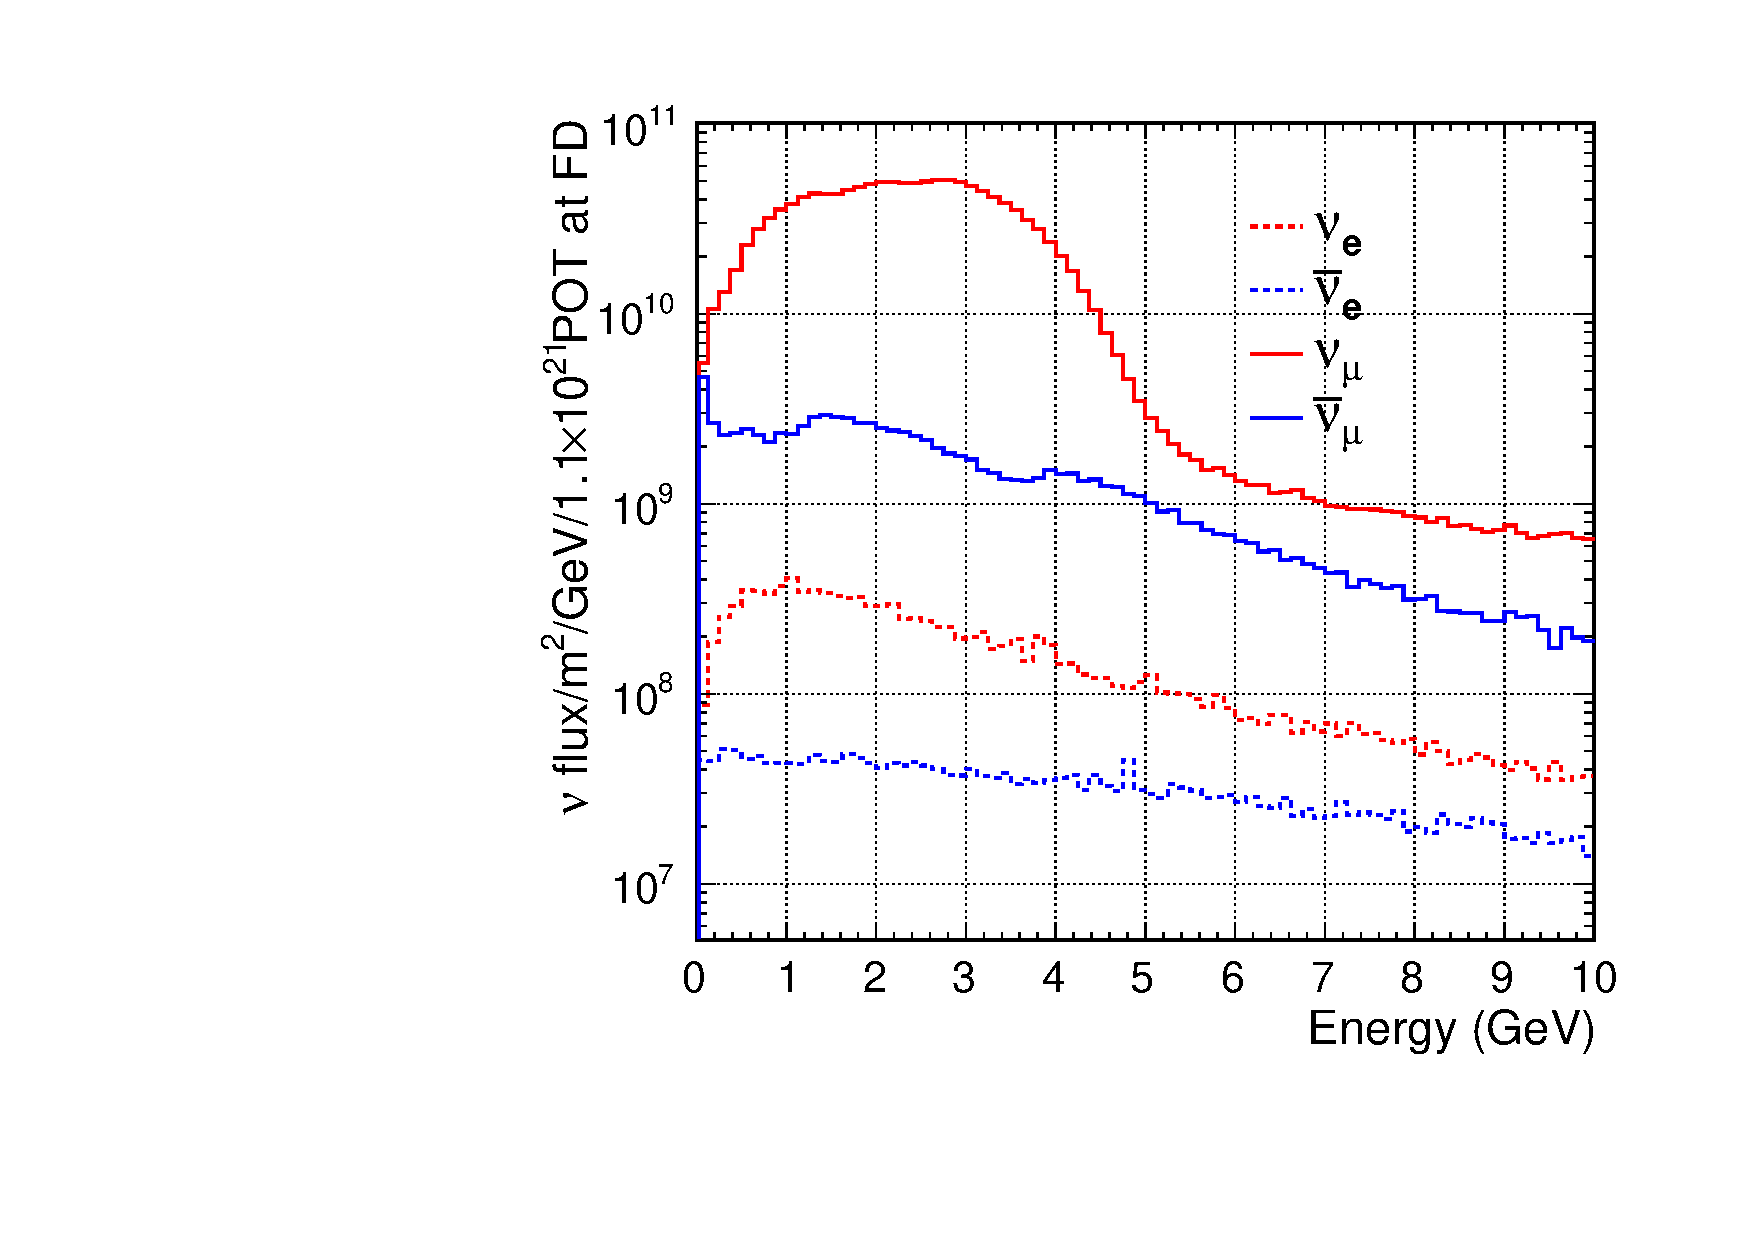
\includegraphics[width=.99\linewidth]{Images/DUNE/LBNF/dune_neutrino_fd_log}
	\end{subfigure}
	\begin{subfigure}{0.49\textwidth}
		\centering
		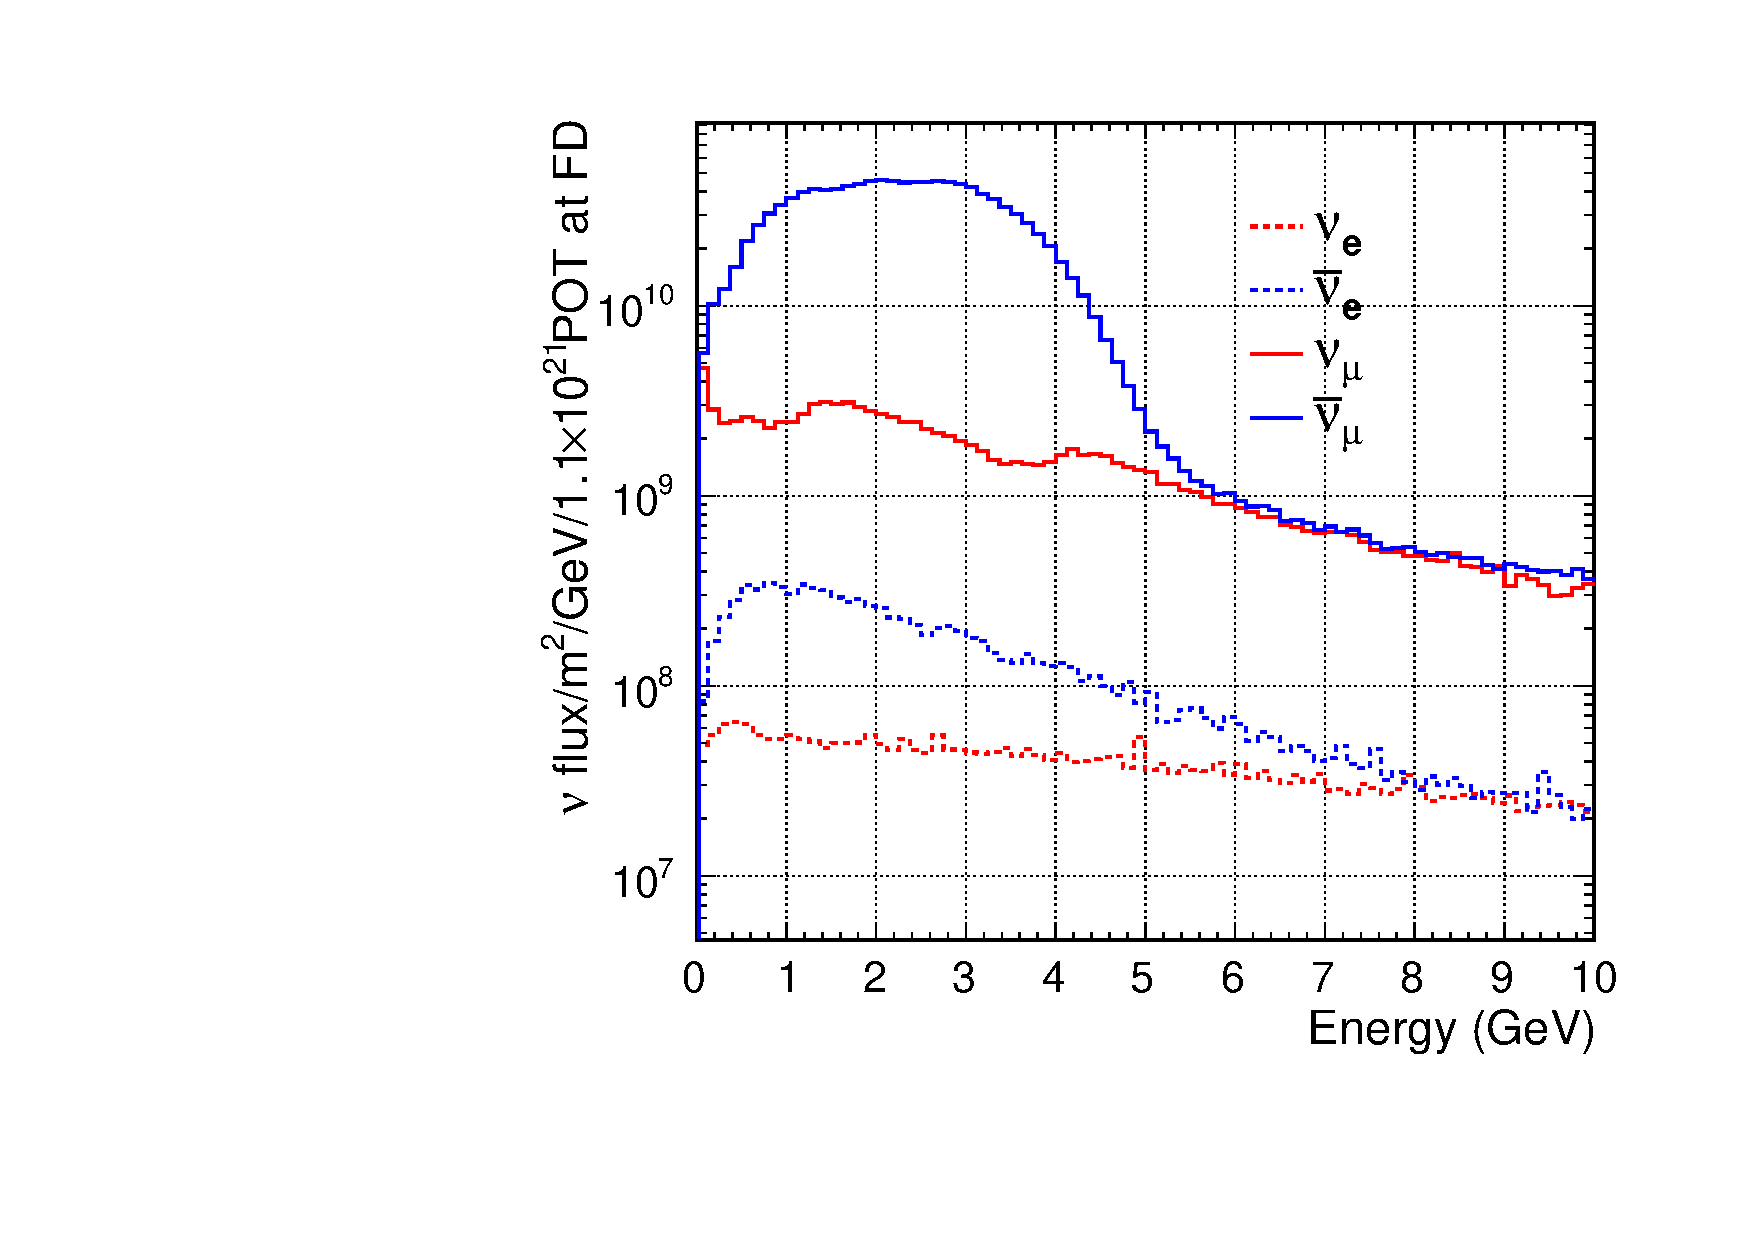
\includegraphics[width=.99\linewidth]{Images/DUNE/LBNF/dune_antineutrino_fd_log}
	\end{subfigure}
	\caption[Predicted neutrino fluxes at the FD in FHC mode and RHC mode.]{Predicted neutrino fluxes at the FD in FHC mode (left panel) and RHC mode (right panel). Figures taken from Ref. \cite{DUNE2020TDR2}.}
	\label{fig:dune_fd_flux}
\end{figure}

\section{Near Detector}

To estimate the oscillation parameters we measure the neutrino energy spectra at the FD. This reconstructed energy arises from a convolution of the neutrino flux, cross section, detector response and the oscillation probability. Using theoretical and empirical models to account for the other effects, one can extract the oscillation probability using the measurement. However, these models have associated a number of uncertainties that are then propagated to the oscillation parameters.

\begin{figure}[t]
	\centering
	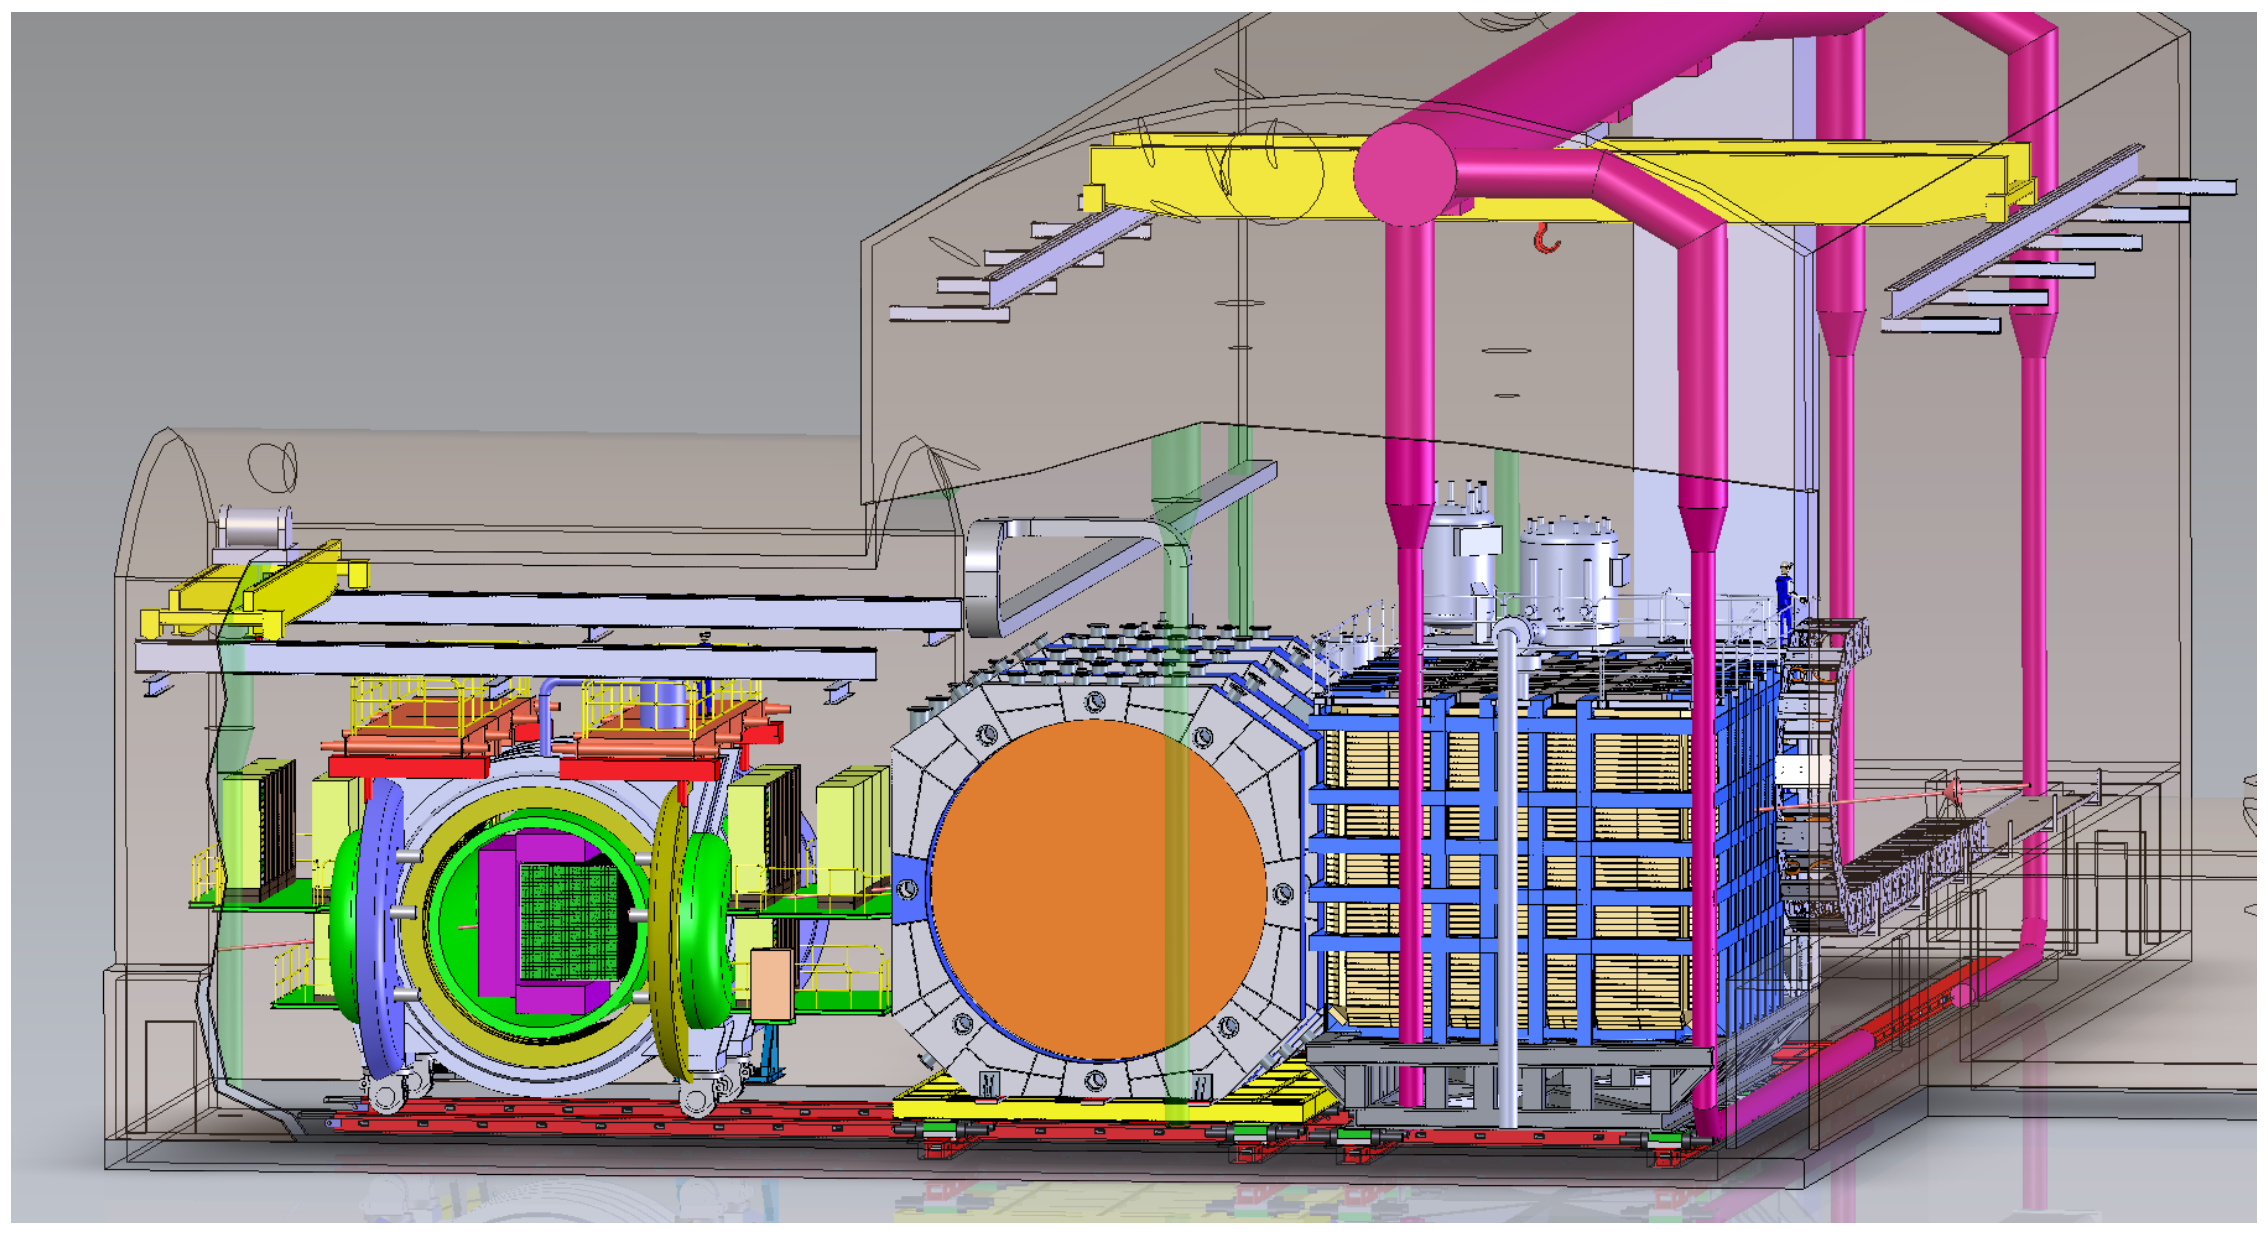
\includegraphics[width=0.95\linewidth]{Images/DUNE/ND/nd_hall}
	\caption[Representation of the ND hall in Phase II, showing the different subcomponents.]{Representation of the ND hall in Phase II, showing the different subcomponents. From right to left, in the direction of the beam, we have ND-LAr, ND-GAr and SAND. Figure taken from Ref. \cite{DUNE2021NDCDR}.}
	\label{fig:dune_nd}
\end{figure}

One of the main roles of the ND is to measure the neutrino interaction rates before the oscillation effects become relevant, i.e. close to the production point. By measuring the $\nu_{\mu}$ and $\nu_{e}$ energy spectra, and that of their corresponding antineutrinos, at the ND we can constrain the model uncertainties. A complete cancellation of the uncertainties when taking the ratio between the FD and ND measurements is not possible, as that would require both detectors to have identical designs and the neutrino fluxes to be the same. Because of the distance, the flux probed by the FD will have a different energy and flavour composition than that at the ND, as neutrinos oscillate and the beam spreads. The differences in the flux also determine the design of the detectors, therefore the ND is limited in its capability to match the FD design.

Nevertheless, having a highly capable ND, DUNE can minimise the systematic uncertainties affecting the observed neutrino energy. The ND data can be used to tune the model parameters by comparison with the prediction. Then, one uses the tuned model to predict the unoscillated FD spectra. Comparing the prediction with the measured spectra it is possible to extract the oscillation parameters.

\begin{comment}
	Another requirement for the ND is that it must reduce the impact of the cross section uncertainties on the measurement of the neutrino spectra. In other words, it needs to measure neutrino interactions much more accurately than the FD. This requires a better particle identification and energy reconstruction capabilities.
\end{comment}

\begin{figure}[t]
	\centering
	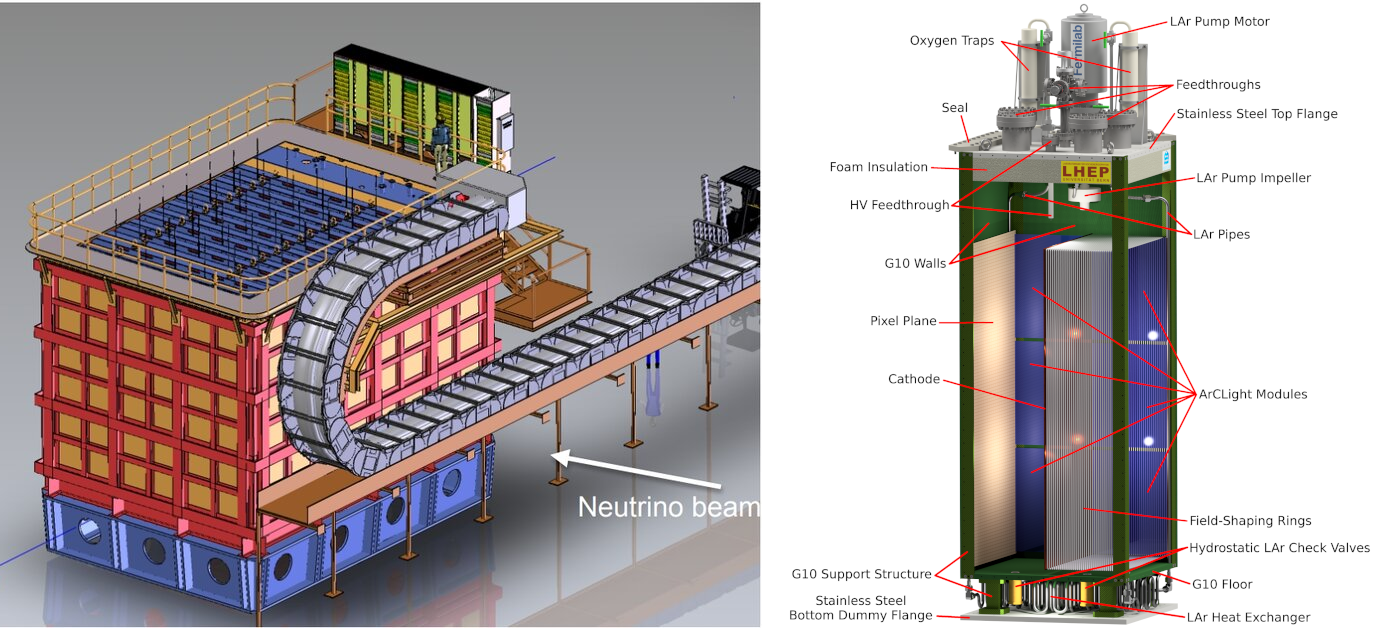
\includegraphics[width=0.99\linewidth]{Images/DUNE/ND/nd_lar_mod}
	\caption[Schematic representation of the external components of ND-LAr, including the cryostat and the PRISM movable system and detailed drawing of one ArgonCube module.]{Schematic representation of the external components of ND-LAr, including the cryostat and the PRISM movable system (left) and detailed drawing of one ArgonCube module (right). Figure adapted from Ref. \cite{DUNE2020TDR1}.}
	\label{fig:dune_nd_lar}
\end{figure}

Additionally, the ND will have a physics program of its own. In particular, it will measure neutrino cross sections that will then be used to constrain the model used in the long-baseline oscillation analysis. It will also be used to search for BSM phenomena such as heavy neutral leptons, dark photons, millicharged particles, etc.

The DUNE ND can be divided in three main components, a LArTPC known as ND-LAr, a magnetised muon spectrometer, which will be the Temporary Muon Spectrometer (TMS) in Phase I and ND-GAr in Phase II, and the System for on-Axis Neutrino Detection (SAND). The layout of the Phase II DUNE ND can be seen in Fig. \ref{fig:dune_nd}. The first two components of the ND will be able to move off-axis, in what is called the Precision Reaction-Independent Spectrum Measurement (PRISM) concept. More details on the purpose and design of the ND can be found in the DUNE ND Conceptual Design Report (CDR) \cite{DUNE2021NDCDR}.

\subsection{ND-LAr}

\begin{figure}[t]
	\centering
	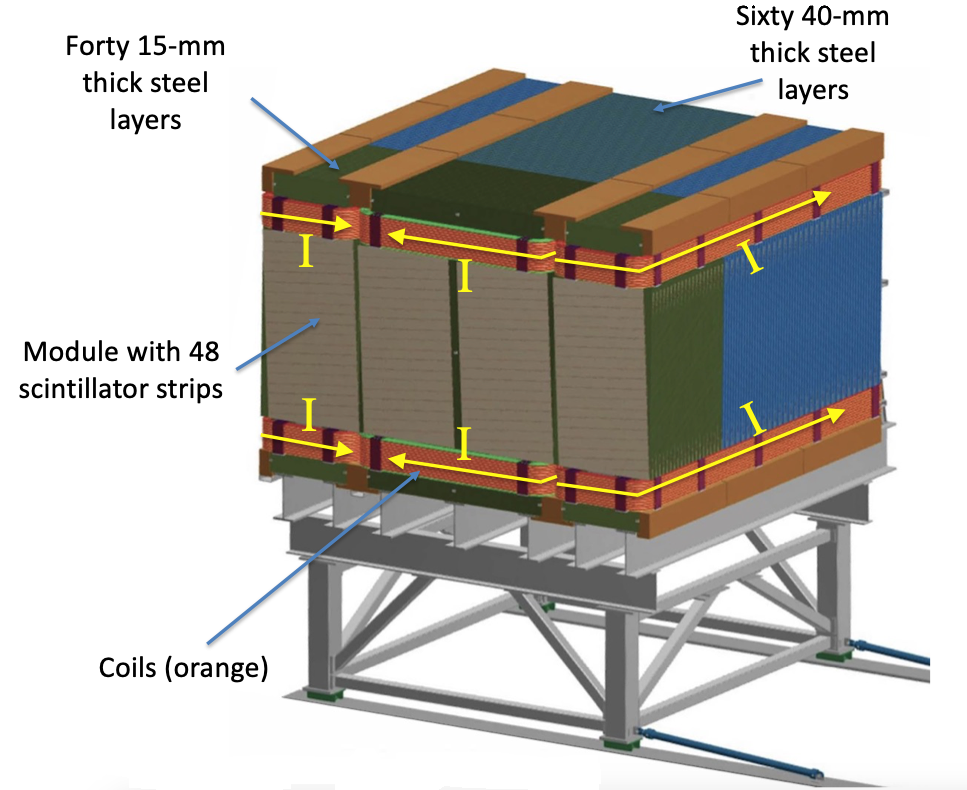
\includegraphics[width=0.65\linewidth]{Images/DUNE/ND/nd_tms}
	\caption[Schematic view of the TMS detector, highlighting its main parts.]{Schematic view of the TMS detector, highlighting its main parts. Figure adapted from Ref. \cite{DUNE2020TDR1}.}
	\label{fig:dune_tms}
\end{figure}

ND-LAr is a LArTPC, as the ND needs a LAr component to reduce cross section and detector systematic uncertainties in the oscillation analysis. However, its design differs significantly from those proposed for the FD modules. Because of the high event rates at the ND, approximately $55$ neutrino interaction events per $10~\mu\mathrm{s}$ spill, ND-LAr will be built in a modular way. Each of the modules, based on the ArgonCube technology, is a fully instrumented, optically isolated TPC with a pixelated readout. The pixelisation allows for a fully 3D reconstruction and the optical isolation reduces the problems due to overlapping interactions. Figure \ref{fig:dune_nd_lar} shows a representation of the external parts of ND-LAr (left) and a detailed diagram of an ArgonCube module (right).

With a fiducial mass of $67~\mathrm{t}$ and dimensions $7~\mathrm{m} \ (\text{w}) \times 3~\mathrm{m} \ (\text{h}) \times 5~\mathrm{m} \ (\text{l})$, ND-LAr will be able to provide high statistics and contain the hadronic systems from the beam neutrino interactions, but muons with a momentum higher than $0.7~\mathrm{GeV}$ will exit the detector.

\begin{figure}[t]
	\centering
	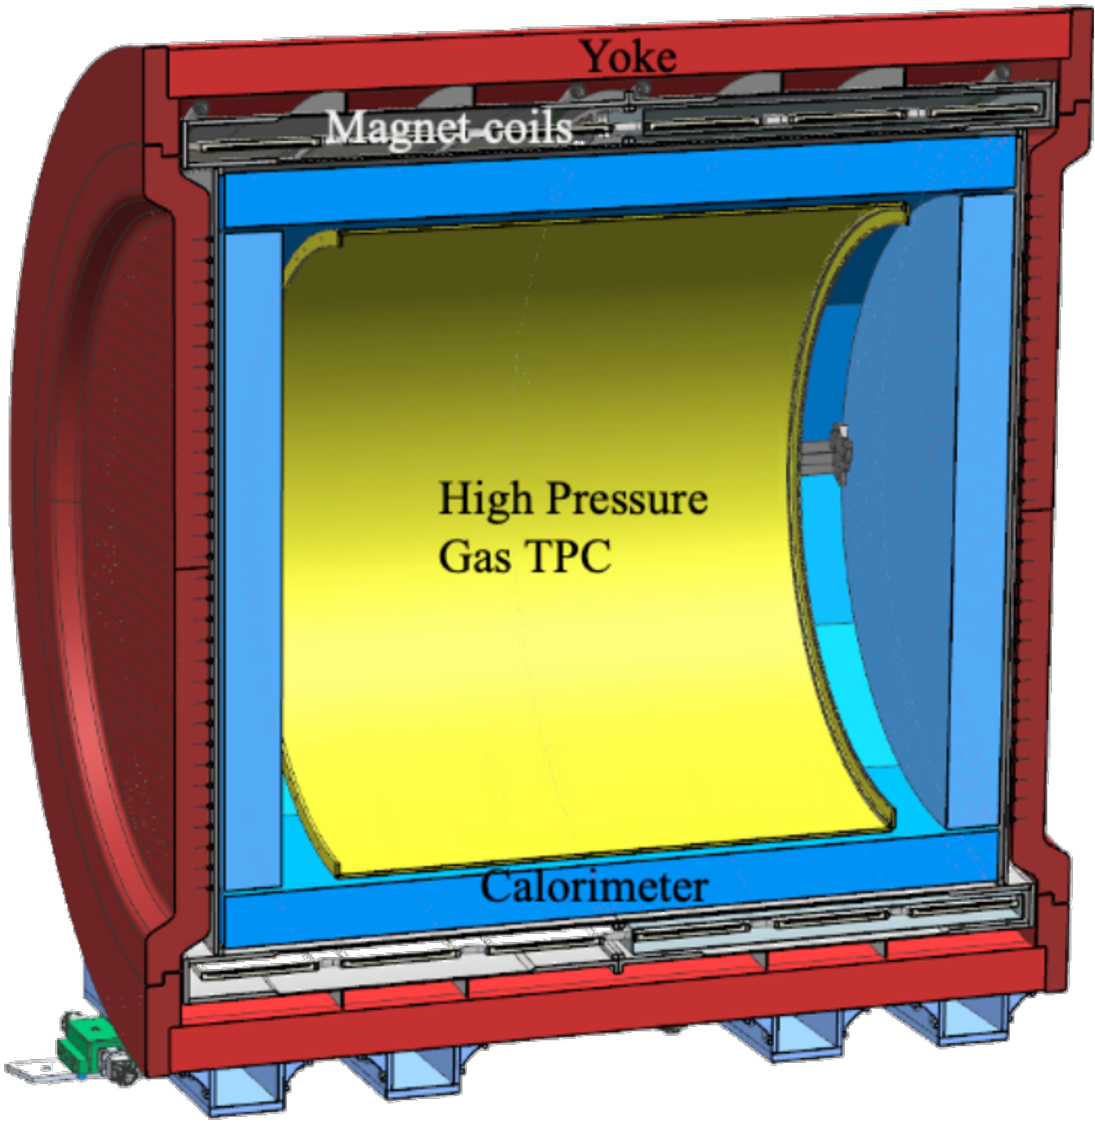
\includegraphics[width=0.45\linewidth]{Images/DUNE/ND/nd_gar}
	\caption[Cross section of the ND-GAr geometry, showing the HPgTPC, ECal and magnet.]{Cross section of the ND-GAr geometry, showing the HPgTPC, ECal and magnet. Figure adapted from Ref. \cite{DUNE2024Phase2}.}
	\label{fig:dune_nd_gar}
\end{figure}

\subsection{TMS/ND-GAr}

To accurately estimate the neutrino energy, the momentum of the outgoing muons needs to be determined. That is the reason why a muon spectrometer is needed downstream of ND-LAr.

In Phase I that role will be fulfilled by TMS. It is a magnetised sampling calorimeter, with alternating steel and plastic scintillator layers. Figure \ref{fig:dune_tms} shows a schematic view of the TMS detector. The magnetic field allows a precise measurement of the sign of the muon, so one can distinguish between neutrino and antineutrino interactions.

After the Phase II upgrade, TMS will be replaced with a more capable near detector. The current technology considered is ND-GAr. This detector is a magnetised, high-pressure GAr TPC (often denoted as HPgTPC) surrounded by an electromagnetic calorimeter (ECal) and a muon tagger. A cross section of its geometry can be seen in Fig. \ref{fig:dune_nd_gar}. ND-GAr will be able to measure the momenta of the outgoing muons while also detect neutrino interactions inside the GAr volume. This allows ND-GAr to constrain the systematic uncertainties even further, as it will be able to accurately measure neutrino interactions at low energies thanks to the lower tracking thresholds of GAr.

\begin{figure}[t]
	\centering
	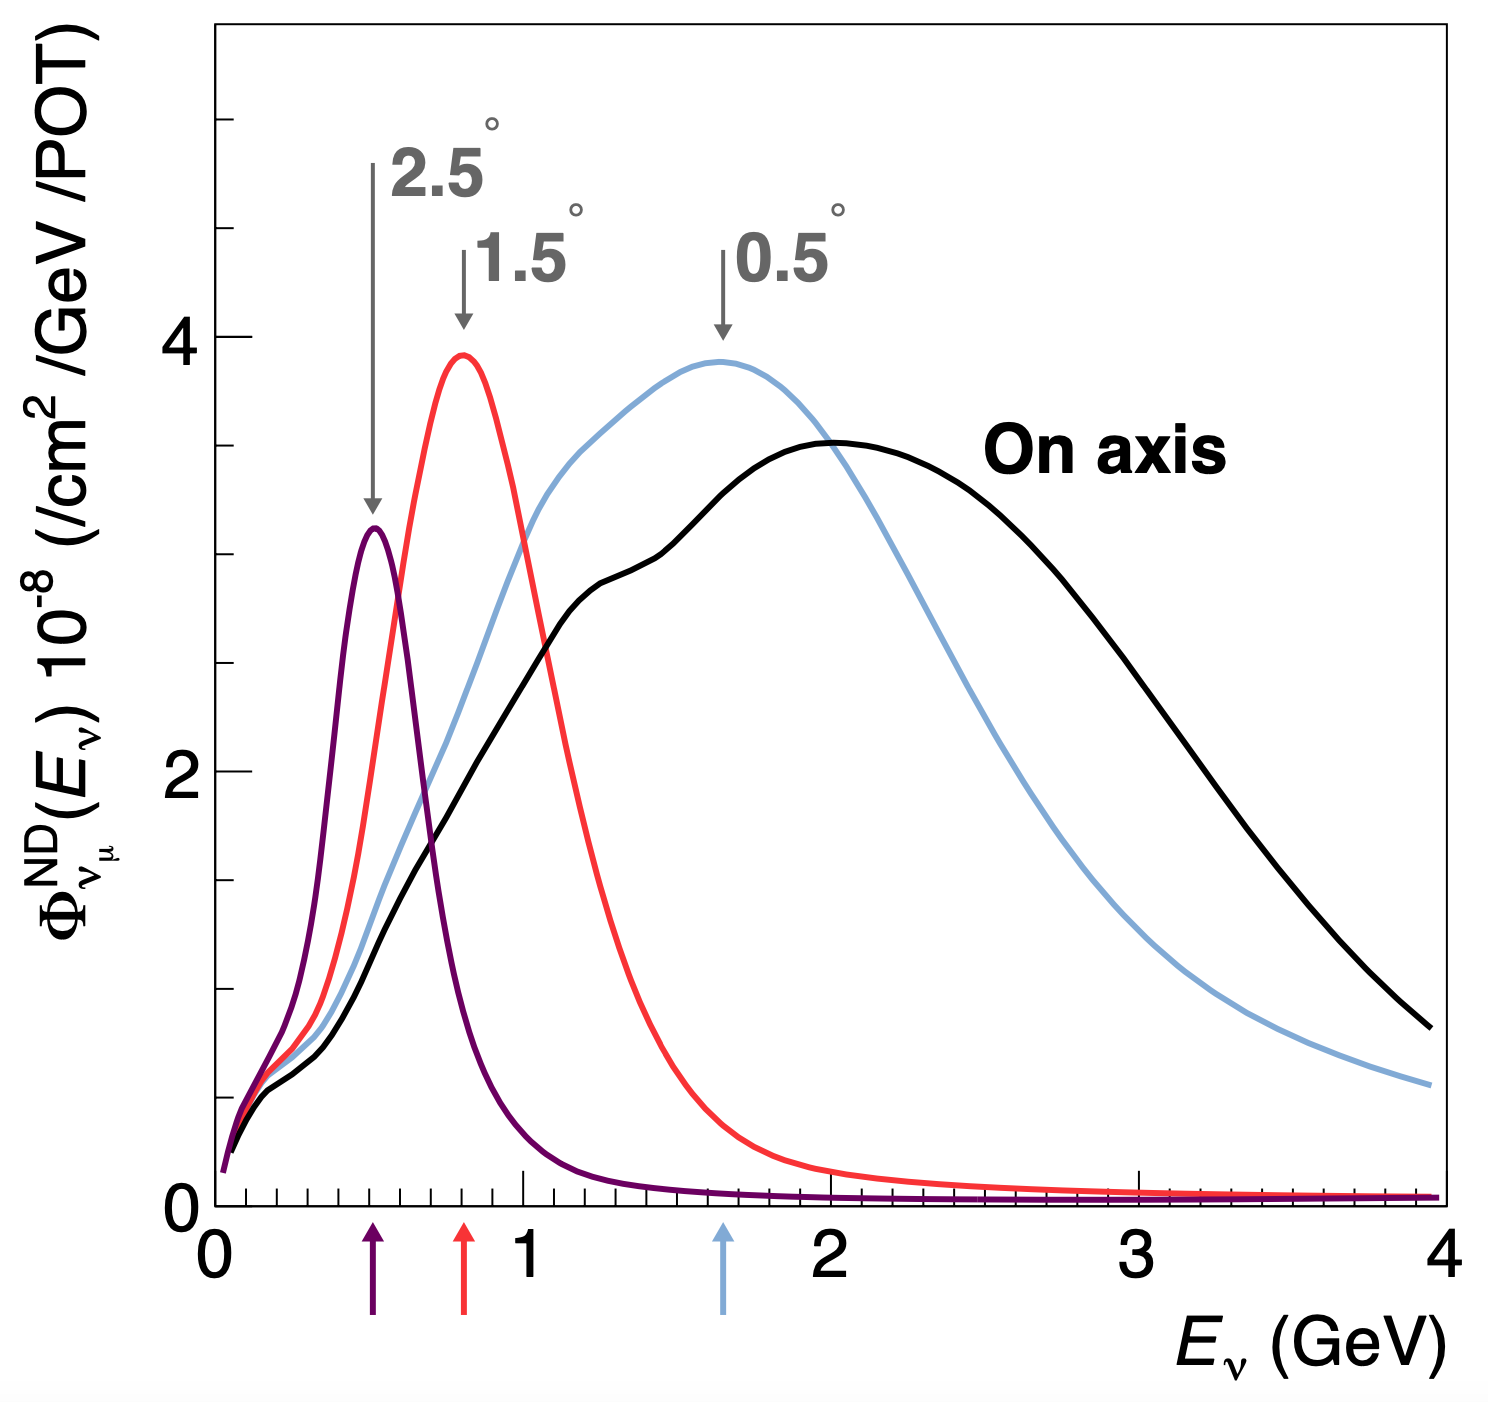
\includegraphics[width=0.55\linewidth]{Images/DUNE/ND/prism_spectra}
	\caption[Predicted beam muon neutrino flux at the ND location for different off-axis positions.]{Predicted beam muon neutrino flux at the ND location for different off-axis positions. Figure taken from Ref. \cite{DUNE2021NDCDR}.}
	\label{fig:dune_prism}
\end{figure}

\subsection{PRISM}

In general, the observed peak neutrino energy of a neutrino beam decreases as the observation angle with respect to the beam direction increases. This feature has been used in other long-baseline neutrino experiments, like T2K ($2.5^{\circ}$ off-axis) and NOvA ($0.8^{\circ}$ off-axis), to achieve narrower energy distributions. The DUNE PRISM concept exploits this effect using a movable ND. Within PRISM both ND-LAr and the muon spectrometer (TMS in Phase I and ND-GAr in Phase II) can be moved up to $3.2^{\circ}$ off-axis, equivalent to move the detectors $30.5~\mathrm{m}$ laterally through the ND hall.

This allows to record additional data samples with different energy compositions. Figure \ref{fig:dune_prism} compares the on-axis muon neutrino flux at the ND with the fluxes at different off-axis positions. As the off-axis position increases the neutrino flux becomes closer to a monoenergetic beam with a lower peak energy. These samples can be used to perform a data-driven determination of the relation between true and reconstructed neutrino energy, to reduce the dependence on the interaction model. The off-axis samples are linearly combined to produce a narrow Gaussian energy distribution centered on a target true energy. From the combination coefficients one can build a sample of reconstructed neutrino events that will determine the energy mapping.

The PRISM samples will be used to form a flux at the ND location similar in shape to the oscillated flux measured by the FD. This method can be used to extract the oscillation parameters with minimal input from the neutrino interaction model.

\subsection{SAND}

The role of SAND is to monitor the beam stability by measuring the on-axis neutrino energy spectra. As the PRISM program requires that ND-LAr and its downstream muon spectrometer spend about half of the time in off-axis positions, it is not possible to monitor the stability with the movable detectors. Moreover, for the success of PRISM it is essential to have a stable beam configuration, or, at least, a quick assessment and modeling of the distortions.

The SAND detector is magnetised, and features an inner low density tracker, a LAr target with optical readout and surrounding sampling calorimeter.

\section{A More Capable Near Detector}\label{sec:mcnd}

In DUNE Phase II, a more capable near detector is needed to achieve the ultimate physics goals of the experiments. The current leading proposal for this detector is ND-GAr. As mentioned previously, it will fulfill the role of TMS, measuring the momentum and sign of the charged particles exiting ND-LAr. Additionally, it will be able to measure neutrino interactions inside the HPgTPC, achieving lower energy thresholds than those of the ND and FD LArTPCs. By doing so ND-GAr will allow to constrain the relevant systematic uncertainties for the LBL analysis even further. A detailed discussion on the requirements, design, performance and physics of ND-GAr can be found in the DUNE ND CDR \cite{DUNE2021NDCDR} and the ND-GAr white paper \cite{DUNE2022GArWhite}.

\subsection{Requirements}

The primary requirement for ND-GAr is to the measure the momentum and charge of muons from $\nu_{\mu}$ and $\bar{\nu}_{\mu}$ CC interactions in ND-LAr, in order to measure their energy spectrum. To achieve the sensitivity to the neutrino oscillation parameters described in the DUNE FD TDR Volume II \cite{DUNE2020TDR2}, ND-GAr should be able to constrain the muon energy within a $1\%$ uncertainty or better.

Another requirement for ND-GAr is the precise measurement of neutrino interactions on argon for the energies relevant to the neutrino oscillation program. The goal is to constrain the cross section systematic uncertainties in the regions of phase space that are not accessible to ND-LAr. This requires the kinematic acceptance for muons in ND-GAr to exceed that of ND-LAr, being comparable to the one observed in the FD.

ND-GAr should also be able to help establishing the relationship between true and reconstructed energy from neutrino interactions on argon with low thresholds, being sensitive to particles that are not observed or may be misidentified in ND-LAr. In particular, ND-GAr needs to have low tracking thresholds in order to measure the spectrum of pions and protons produced in final-state interactions (FSI). It also must be able to accurately measure the pion multiplicity in 1, 2 and 3 pions final states, to inform the pion mass correction in the LArTPCs.

\subsection{Reference design}

The final design of ND-GAr is still under preparation. However, a preliminary baseline design was in place at the time of the ND CDR. This section summarises the main features of that design, as it is also the one used for the default geometry in our simulation. A DUNE Phase II white paper, discussing the different options under consideration for the ND-GAr design, is in progress. 

\subsubsection{HPgTPC}

The reference design for the ND-GAr HPgTPC follow closely that of the ALICE TPC. It is a cylinder with a central high-voltage cathode, generating the electric field for the two drift volumes, with a maximum drift distance of $2.5~\mathrm{m}$ each. The anodes will be instrumented with charge readout chambers. The original design repurposed the multi-wire proportional readout chambers (MWPCs) of ALICE, however some of the current R\&D efforts focus on a gas electron multiplier (GEM) \cite{Sauli1997} option instead. Figure \ref{fig:alice_tpc} shows a schematic diagram of the ALICE TPC design. The basic ND-GAr geometry will resemble this, except for the inner field cage.

\begin{figure}[t]
	\centering
	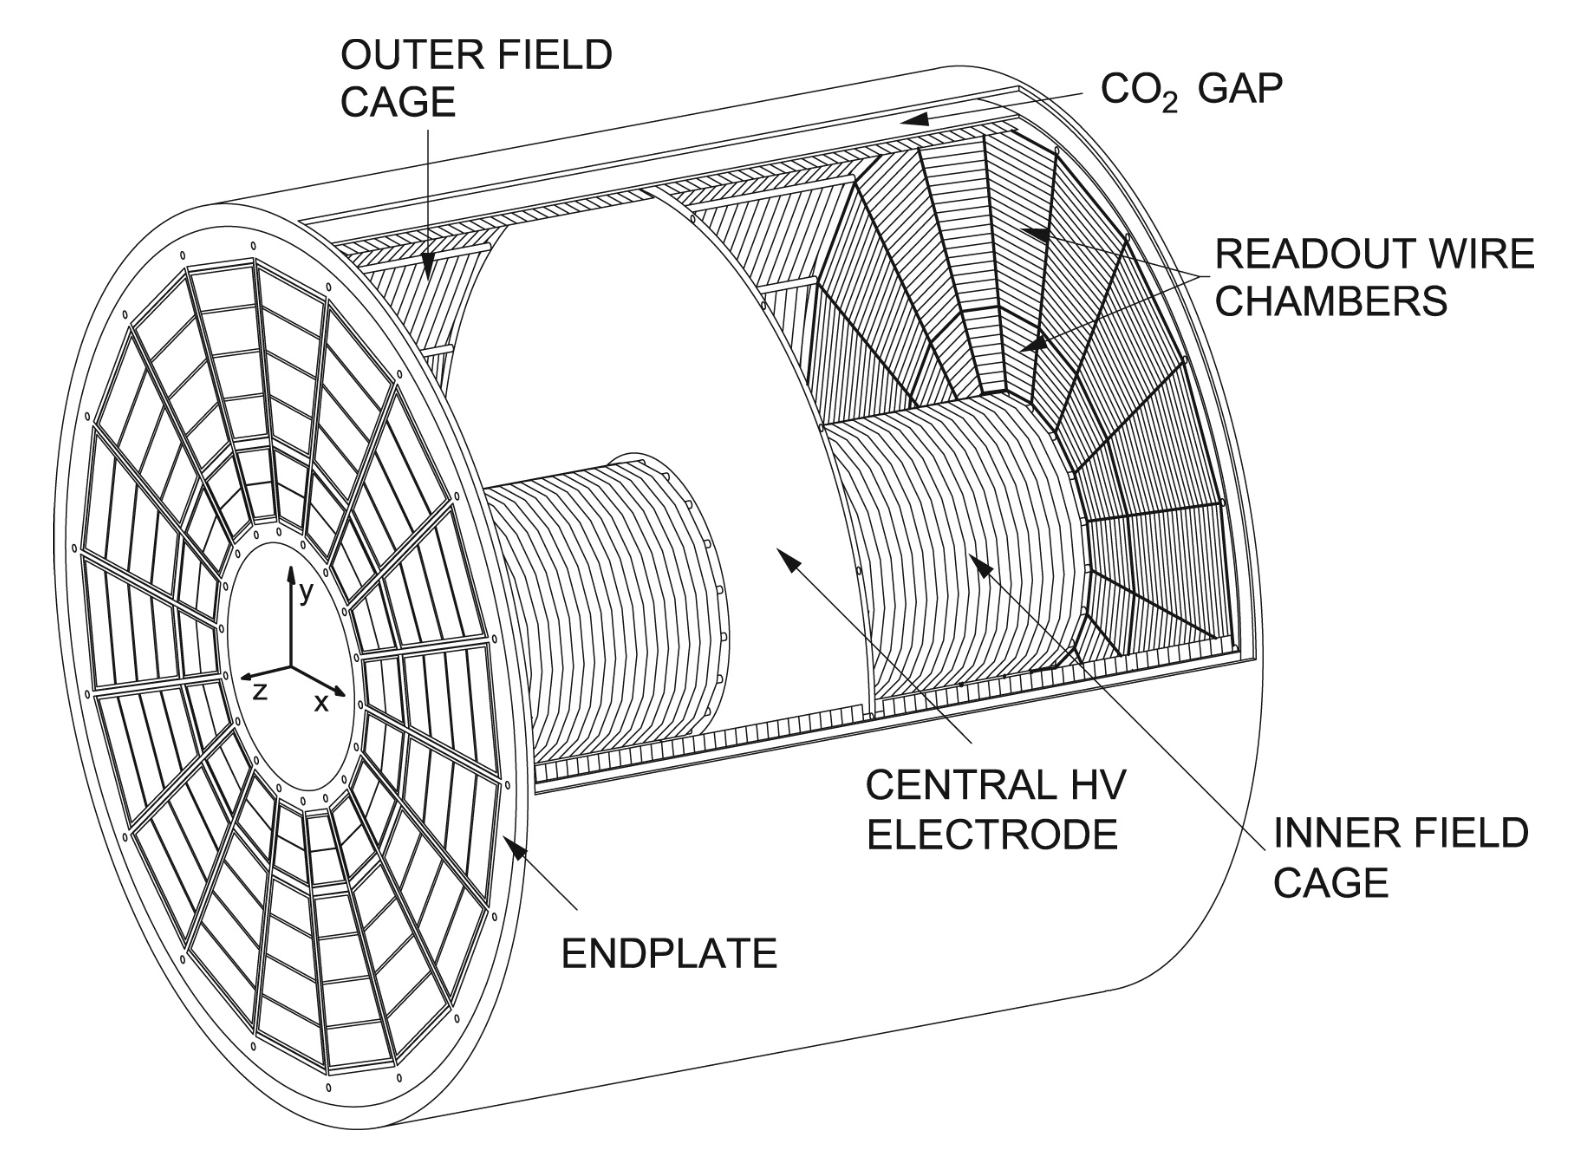
\includegraphics[width=0.7\linewidth]{Images/ND-GAr/alice_tpc}
	\caption[Diagram of the ALICE TPC, showing the two drift chambers, inner and outer field cages and readout chambers.]{Diagram of the ALICE TPC, showing the two drift chambers, inner and outer field cages and readout chambers. Figure taken from Ref. \cite{DUNE2021NDCDR}.}
	\label{fig:alice_tpc}
\end{figure}

It will use a 90:10 molar fraction $\mathrm{Ar}$:$\mathrm{CH}_{4}$ mixture at $10~\mathrm{bar}$. With this baseline gas mixture light collection is not possible, as the quenching gas absorbs most of the VUV photons. Additional R\&D efforts are underway, to understand if different mixtures allow for the light signal to be used to provide a $t_{0}$ while maintaining stable charge gain.

\subsubsection{ECal}

\begin{figure}[t]
	\centering
	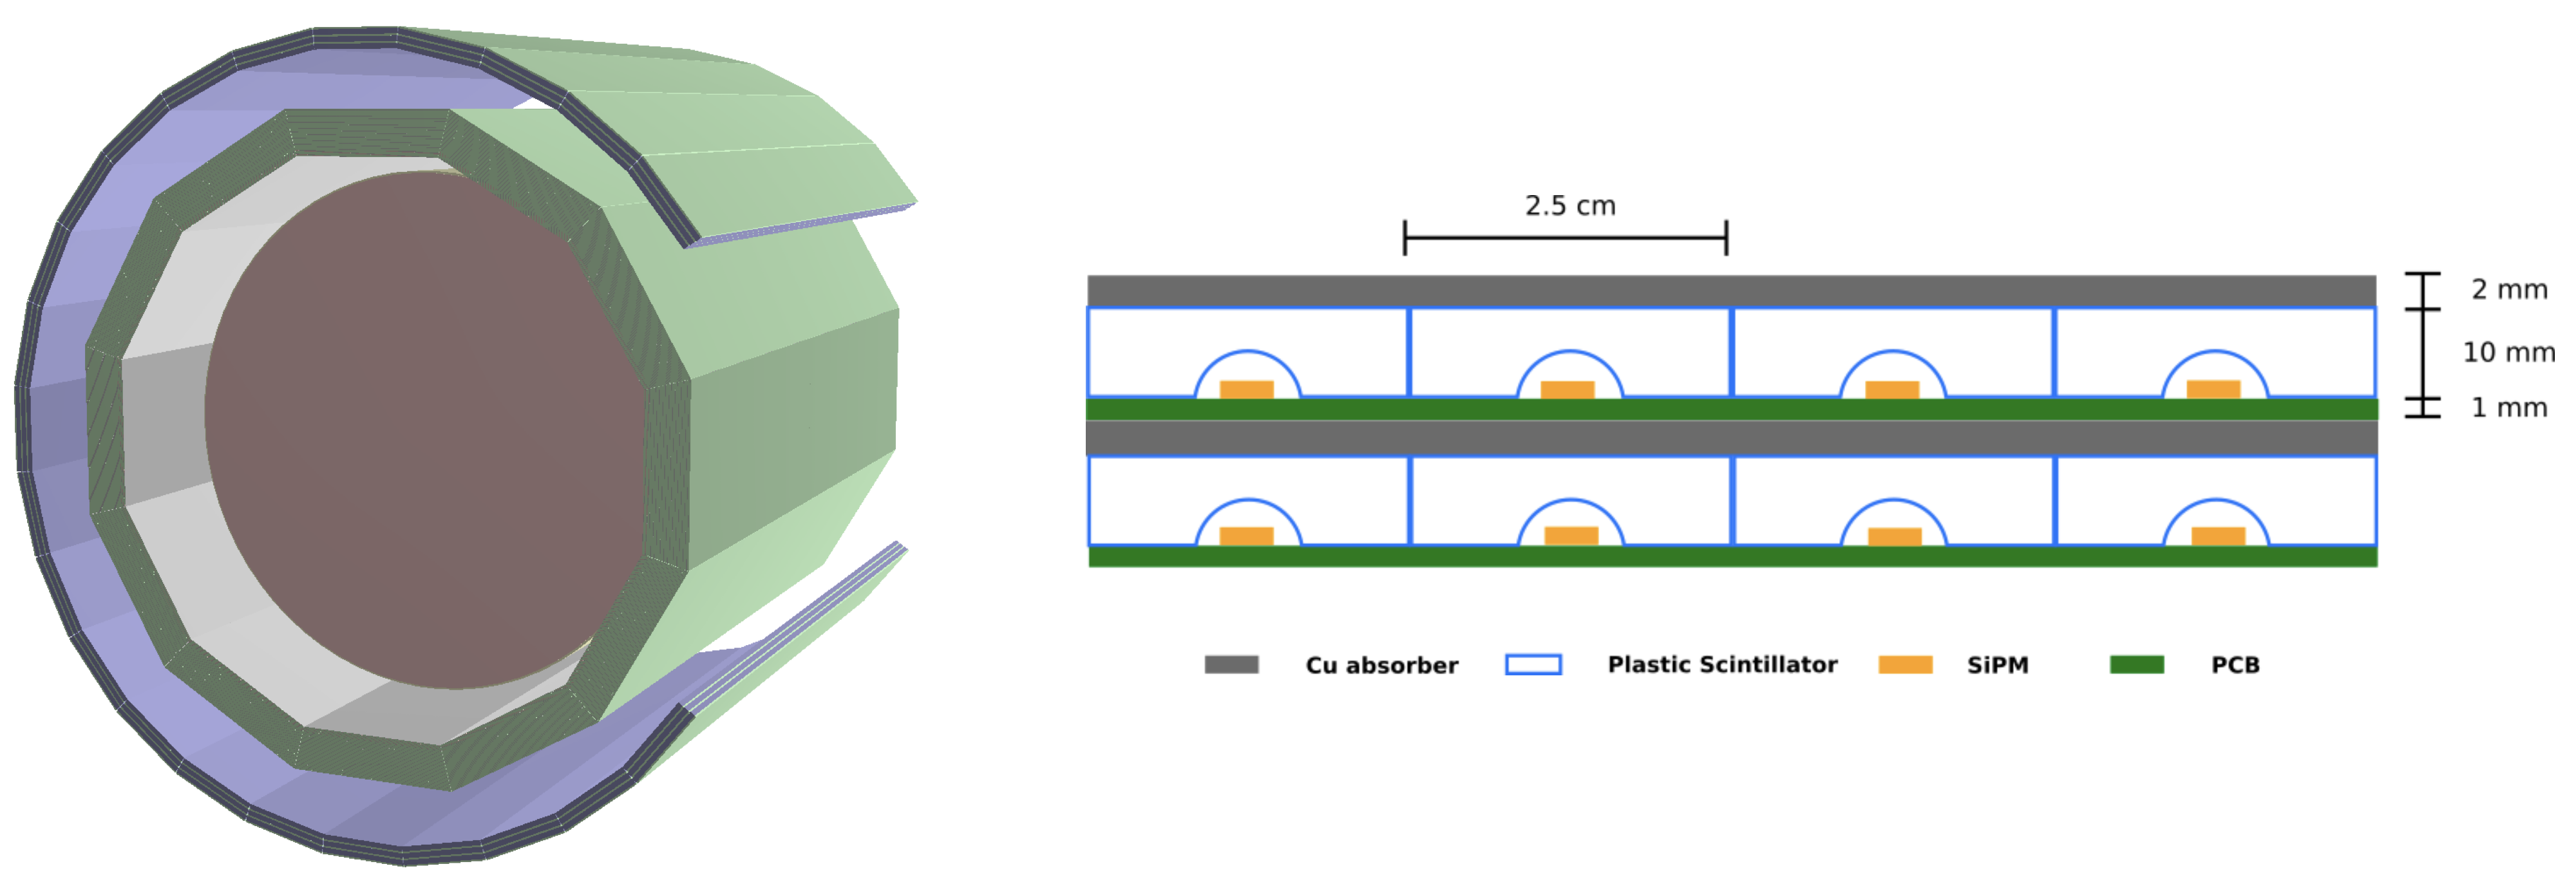
\includegraphics[width=0.99\linewidth]{Images/ND-GAr/ndgar_ecal}
	\caption[Diagram of the ALICE TPC, showing the two drift chambers, inner and outer field cages and readout chambers.]{View of the 12-sided ECal barrel and outer muon tagger geometries (left) and layout of the ECal tile layers for the $2~\mathrm{mm}$ Cu, $10~\mathrm{mm}$ scintillator option (right). Figure adapted from Ref. \cite{DUNE2021NDCDR}.}
	\label{fig:ndgar_ecal}
\end{figure}

The main role of the ND-GAr ECal is the calorimetric measurement of the electron energies and the reconstruction of photons, in particular those from neutral pion decays. Also, the ECal is able to provide a $t_{0}$ timestamp for neutrino interactions, by associating its activity to the tracks in the HPgTPC. The ECal will also be able to perform neutron reconstruction using time of flight and reject external backgrounds, thanks to its sub-nanosecond time resolution.

The ECal design features three independent subdetectors, two end caps at each side and a barrel surrounding the HPgTPC. Each of the detectors is divided in modules, which combine alternating layers of plastic scintillator and absorber material readout by SiPMs. The inner scintillator layers consist of $2.5\times2.5~\mathrm{cm}^{2}$ high-granularity tiles, whereas the outer ones are made out of $4~\mathrm{cm}$ wide cross-strips spanning the whole module length. The current barrel geometry consists of 8 tile layers and 34 strip layers, while the end caps feature 6 and 36 respectively. The thickness of the scintillator layers is $7~\mathrm{mm}$ and $5~\mathrm{mm}$ for the Pb absorber layers. The 12-sided geometry of the ECal barrel (left) and the layout of the tile layers (left)\footnote{The figure shows the layout of the tile layers for a previous design with $2~\mathrm{mm}$ Cu absorber and $10~\mathrm{mm}$ plastic scintillator, as mentioned in the text the current choice is $5~\mathrm{mm}$ Pb absorber and $7~\mathrm{mm}$ scintillator.} can be seen in Fig. \ref{fig:ndgar_ecal}.

\subsubsection{Magnet}

The ND-GAr magnet design, know as the Solenoid with Partial Yoke (SPY), consists of two coupled solenoids with an iron return yoke. The idea behind the design is to have a solenoid as thin as possible, as well as a return yoke mass distribution that minimises the material budget between ND-LAr and ND-GAr. The magnet needs to provide a $0.5~\mathrm{T}$ field in the direction perpendicular to the beam, parallel to the drift electric field. It needs to host the pressure vessel and the surrounding ECal, which points to a inner diameter of $\sim6.4~\mathrm{m}$.

The solenoid is a single layer coil, based on niobium titanium superconducting Rutherford cable. The total length of the coil is $7.5~\mathrm{m}$. The bobbin will be split in four segments grouped in pairs with two identical cryostats, connected in series. The iron yoke features an aperture in the upstream side to allow the muons coming from ND-LAr. Still, its material will be enough to reduce the magnetic field reaching SAND, and also stop the charged pions produced inside the HPgTPC.

\subsubsection{Muon system}

The design of the ND-GAr muon system is still in a preliminary stage. Its role is to distinguish between muons and pions punching through the ECal. This is especially important for wrong-sign determination, to separate these from neutral current events.

In its current form, the muon system consists of three layers of longitudinal sampling structures. It alternates $10~\mathrm{cm}$ Fe absorber slabs with $2~\mathrm{cm}$ plastic scintillator strips. The transverse granularity required is still under study.

\subsection{R\&D efforts}

\begin{figure}[t]
	\centering
	\includegraphics[width=0.99\linewidth]{Images/ND-GAr/toad.png}
	\caption[Photographs of the TOAD pressure vessel at RHUL.]{Photographs of the TOAD pressure vessel at RHUL. The TPC is mounted inside the vessel, and the OROC is supported by an aluminium frame. Figure taken from Ref. \cite{Ritchie-Yates2023}.}
	\label{fig:toad}
\end{figure}

There are several ND-GAr-related prototypes, mostly focused on the TPC charge readout and electronics. The priority is to test the full readout chain, in a high-pressure environment, using a gas mixture with high argon fraction. A detailed summary of these can be found in the DUNE Phase II white paper \cite{DUNE2024Phase2}.

\subsubsection{Multi-Wire Proportional Chambers}

As mentioned before, the original ND-GAr design repurposes the MWPCs of the ALICE TPC, which became available after the recent upgrade \cite{ALICETPC2020}. These were operated using a 90:10:5 $\mathrm{Ne}$:$\mathrm{CO}_{2}$:$\mathrm{N}_{2}$ gas mixture at $1~\mathrm{atm}$. Therefore, their performance needed to be studied in an argon gas environment at high pressure.

The Gas-argon Operation of ALICE TPC (GOAT) test stand tested the ALICE readout chambers at high pressure. In particular, it used one of the previously operated ALICE inner MWPCs, also known as IROCs, in a pressure vessel rated to $10~\mathrm{atm}$. It measured the gas gain at various pressure points, voltages and gas mixtures.

The Test stand of an Overpressure Argon Detector (TOAD) tested an ALICE outer MWPC, also known as OROC, up to $5~\mathrm{atm}$. During its time at RHUL, it was used to study the achievable gas gain of the OROC \cite{Ritchie-Yates2023}. At the moment, it is being commissioned at Fermilab for a full detector test of the readout electronics and the DAQ.

Figure \ref{fig:toad} shows the interior of the TOAD pressure vessel. The TPC is mounted inside the vessel on three rails. The back of the OROC, supported by an aluminium frame, can be seen at the front.

\begin{figure}[h!]
	\begin{subfigure}{0.49\textwidth}
		\centering
		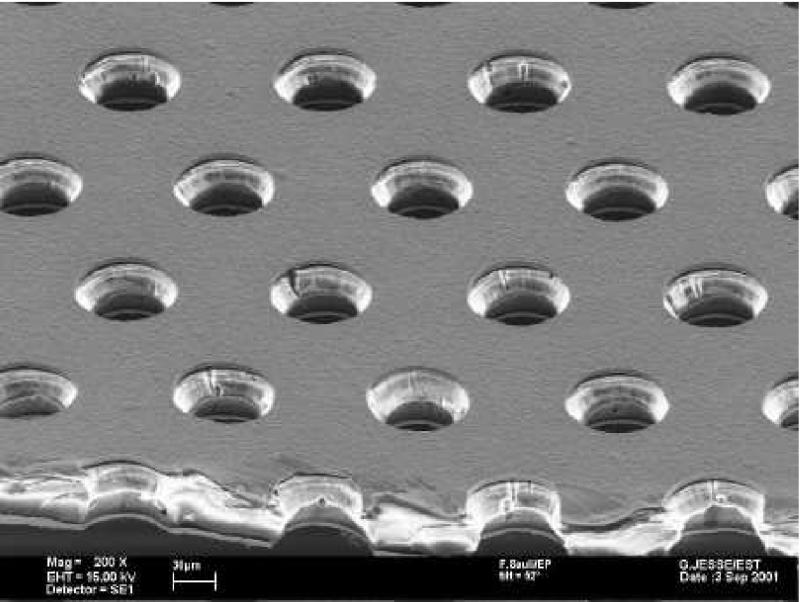
\includegraphics[width=.90\linewidth]{Images/ND-GAr/GEM_photo.jpg}
	\end{subfigure}
	\begin{subfigure}{0.49\textwidth}
		\centering
		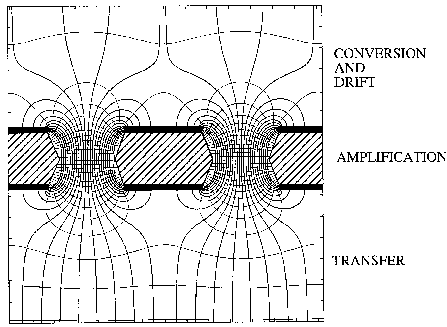
\includegraphics[width=.90\linewidth]{Images//ND-GAr/GEM_diagram.pdf}
	\end{subfigure}
	\caption[Electron microscope image and schematic diagram of a GEM electrode.]{Left panel: electron microscope image of a $50~\mu\mathrm{m}$ thick GEM electrode, with hole pitch and diameter of $140$ and $70~\mu\mathrm{m}$, respectively. Right panel: Schematics of a GEM electrode cross section, showing the electric field lines around the holes. Figures taken from Ref. \cite{Sauli2016}.}
	\label{fig:gem}
\end{figure}

\subsubsection{Gas Electron Multiplier}

An alternative to the MWPC option is the use of GEMs. These are a type of micro-patter detector, where the ionisation electrons passing through the holes in the GEM layers are accelerated by a high intensity electric field. The acceleration causes the electrons to ionise the medium, resulting in an avalanche which increase the signal exponentially \cite{Sauli1997}. GEMs are used in numerous experiments that need a high spatial resolution, like ALICE \cite{Lippmann2016} and CMS \cite{Calabria2016} after their upgrades.

Figure \ref{fig:gem} (left panel) shows an electron microscope picture of a $50~\mu\mathrm{m}$ thick GEM electrode, with a pitch between neighbouring holes of $140~\mu\mathrm{m}$ and a hole diameter of $70~\mu\mathrm{m}$. A schematic representation of the cross section of a GEM layer is shown in Fig. \ref{fig:gem} (left panel).

The Gaseous Argon T0 (GAT0\footnote{Spanish for cat.}) prototype studies the use of thick GEMs made out of glass to achieve optical imaging of the primary ionisation. Using a $10~\mathrm{atm}$ pressure vessel, the goal is to study different argon-based mixtures that allow for a precise $t_{0}$ determination.

The GEM Over-pressurized with Reference Gases (GORG\footnote{Persian for wolf.}) test stand is currently testing a GEM-based charge readout, using a triple-GEM stack.

\section{Far Detector}

\begin{figure}[t]
	\centering
	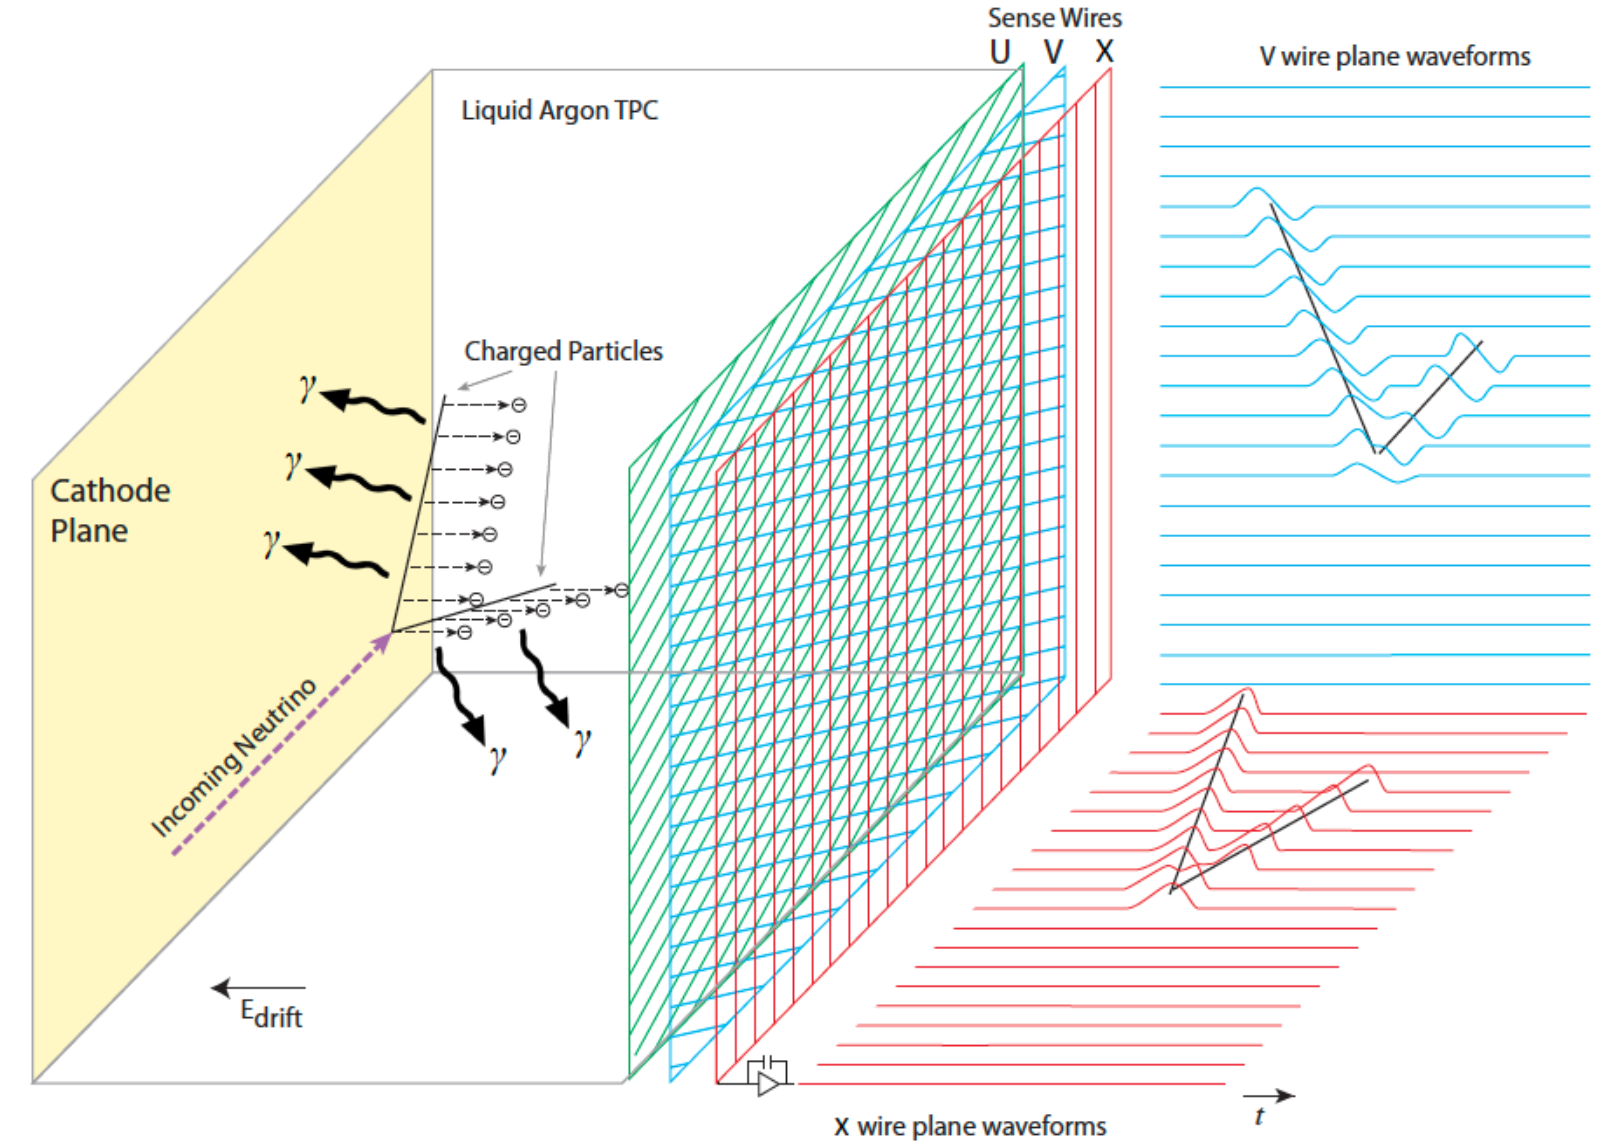
\includegraphics[width=0.8\linewidth]{Images/DUNE/FD/tpc}
	\caption[Schematic diagram showing the operating principle of a LArTPC with wire readout.]{Schematic diagram showing the operating principle of a LArTPC with wire readout. Figure taken from Ref. \cite{DUNE2020TDR1}.}
	\label{fig:lartpc}
\end{figure}

The DUNE FD complex will sit $1300~\mathrm{km}$ away from the beam target and $1.5~\mathrm{km}$ underground at SURF, South Dakota. Two caverns will host the four FD modules, two of them per cavern, each embedded in cryostats of dimensions $18.9~\mathrm{m} \ (\text{w}) \times 17.8~\mathrm{m} \ (\text{h}) \times 65.8~\mathrm{m} \ (\text{l})$. A central, smaller cavern will host the cryogenic system.

Three out of the four modules will be liquid argon (LAr) time projection chamber detectors, often refer to as LArTPCs, with a LAr fiducial mass of at least $10 \ \mathrm{kt}$ each. The first and second FD modules, FD-1 and FD-2, will use a Horizontal Drift (HD) technology, whereas the third module, FD-3, will have a Vertical Drift (VD) direction. The technology for the fourth module is still to be decided, 

For each event, with energies ranging from a few $\mathrm{MeV}$ to several $\mathrm{GeV}$, these detectors collect both the scintillation light and the ionisation electrons created when the charged particles produced in neutrino-nucleus interactions ionise the argon nuclei. In both HD and VD designs the characteristic $128~\mathrm{nm}$ scintillation light of argon is collected by a photon detection system (PDS). This light will indicate the time at which electrons start to drift, thus enabling reconstruction over the drift coordinate when compared to the time when the first ionisation electron arrives to the anode. Reconstruction of the topology in the transverse direction is achieved using the charge readout. Fig. \ref{fig:lartpc} illustrates the detection principle described, for the case of a HD detector with a wire readout.

\subsection{Horizontal Drift}

\begin{figure}[t]
	\centering
	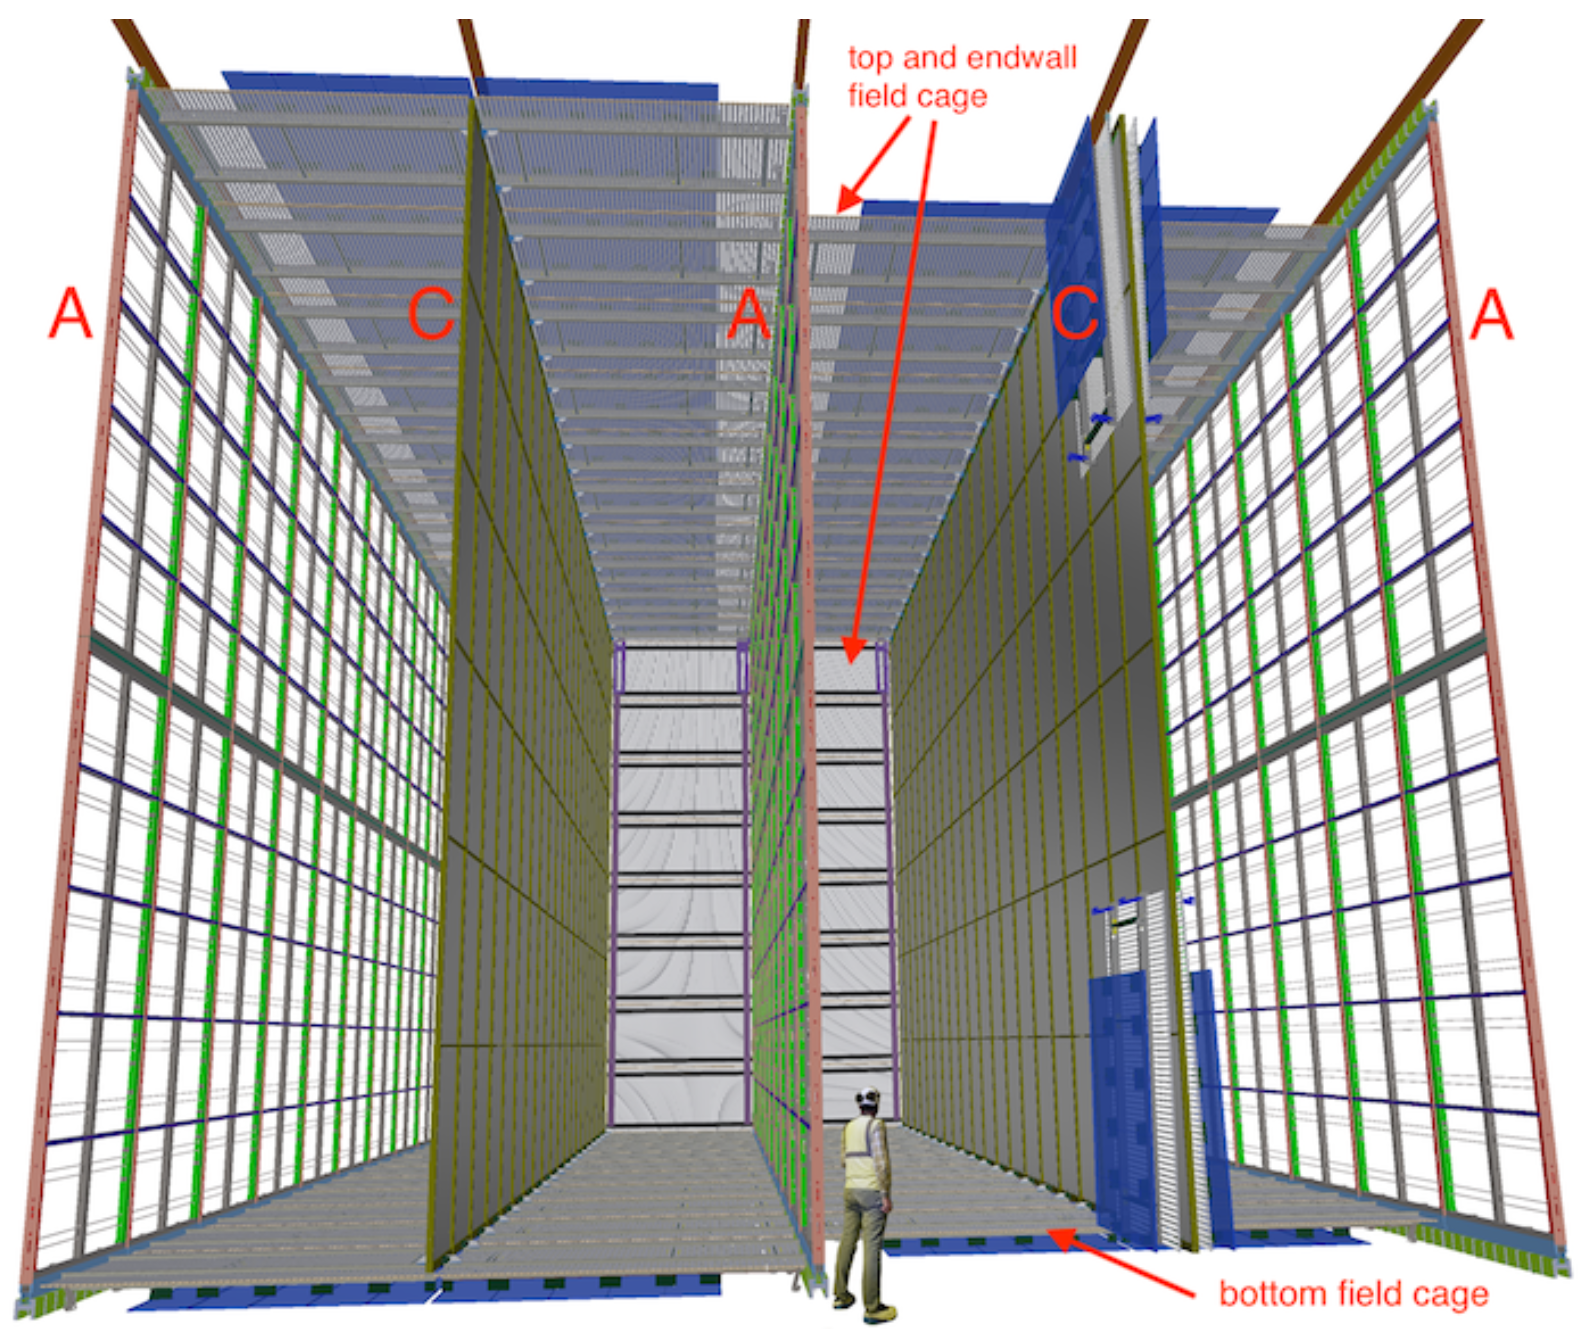
\includegraphics[width=0.65\linewidth]{Images/DUNE/FD/dune_hd}
	\caption[Proposed design for the FD-1 and FD-2 modules following the HD principle.]{Proposed design for the FD-1 and FD-2 modules following the HD principle. Figure taken from Ref. \cite{DUNE2020TDR1}.}
	\label{fig:dune_hd}
\end{figure}

The HD design the ionisation electrons produced as charged particles traverse the LAr drift horizontally towards the anode planes, due to the effect of an electric field. These anode planes are made out of three layers of wire readout. This design, previously known as single-phase (SP), was tested by the ProtoDUNE-SP detector at CERN. The prototype collected data from a hadron beam and cosmic rays, providing high-quality data sets for calibration and performance studies.

Each FD HD detector module is divided in four drift regions, with a maximum drift length of $3.5~\mathrm{m}$, by alternating anode and cathode walls. The surrounding field cage ensures the uniformity of the $500~\mathrm{V/cm}$ horizontal electric field across the drift volumes. The three anode walls, which constitute the charge readout of the detector, are built by stacking anode plane assemblies (APAs), 2 high times 25 wide. The design of the HD modules is shown in Fig. \ref{fig:dune_hd}.

Each APA is made of 2560 active wires arranged in three layers, plus an extra grid layer, wrapped around a metal frame. The two induction wire planes, U and V, sit at $\pm 35.7^{\circ}$ to the vertical on each side of the APA. The collection and shielding plane wires, X and G, run parallel to the vertical direction. The ionisation electrons drift past the induction planes, generating bipolar signals on those wires, and are collected by the collection plane, producing a monopolar positive signal. The spacing between the wires is $\sim 5~\mathrm{mm}$, and it defines the spatial resolution of the APA.

\begin{figure}[t]
	\centering
	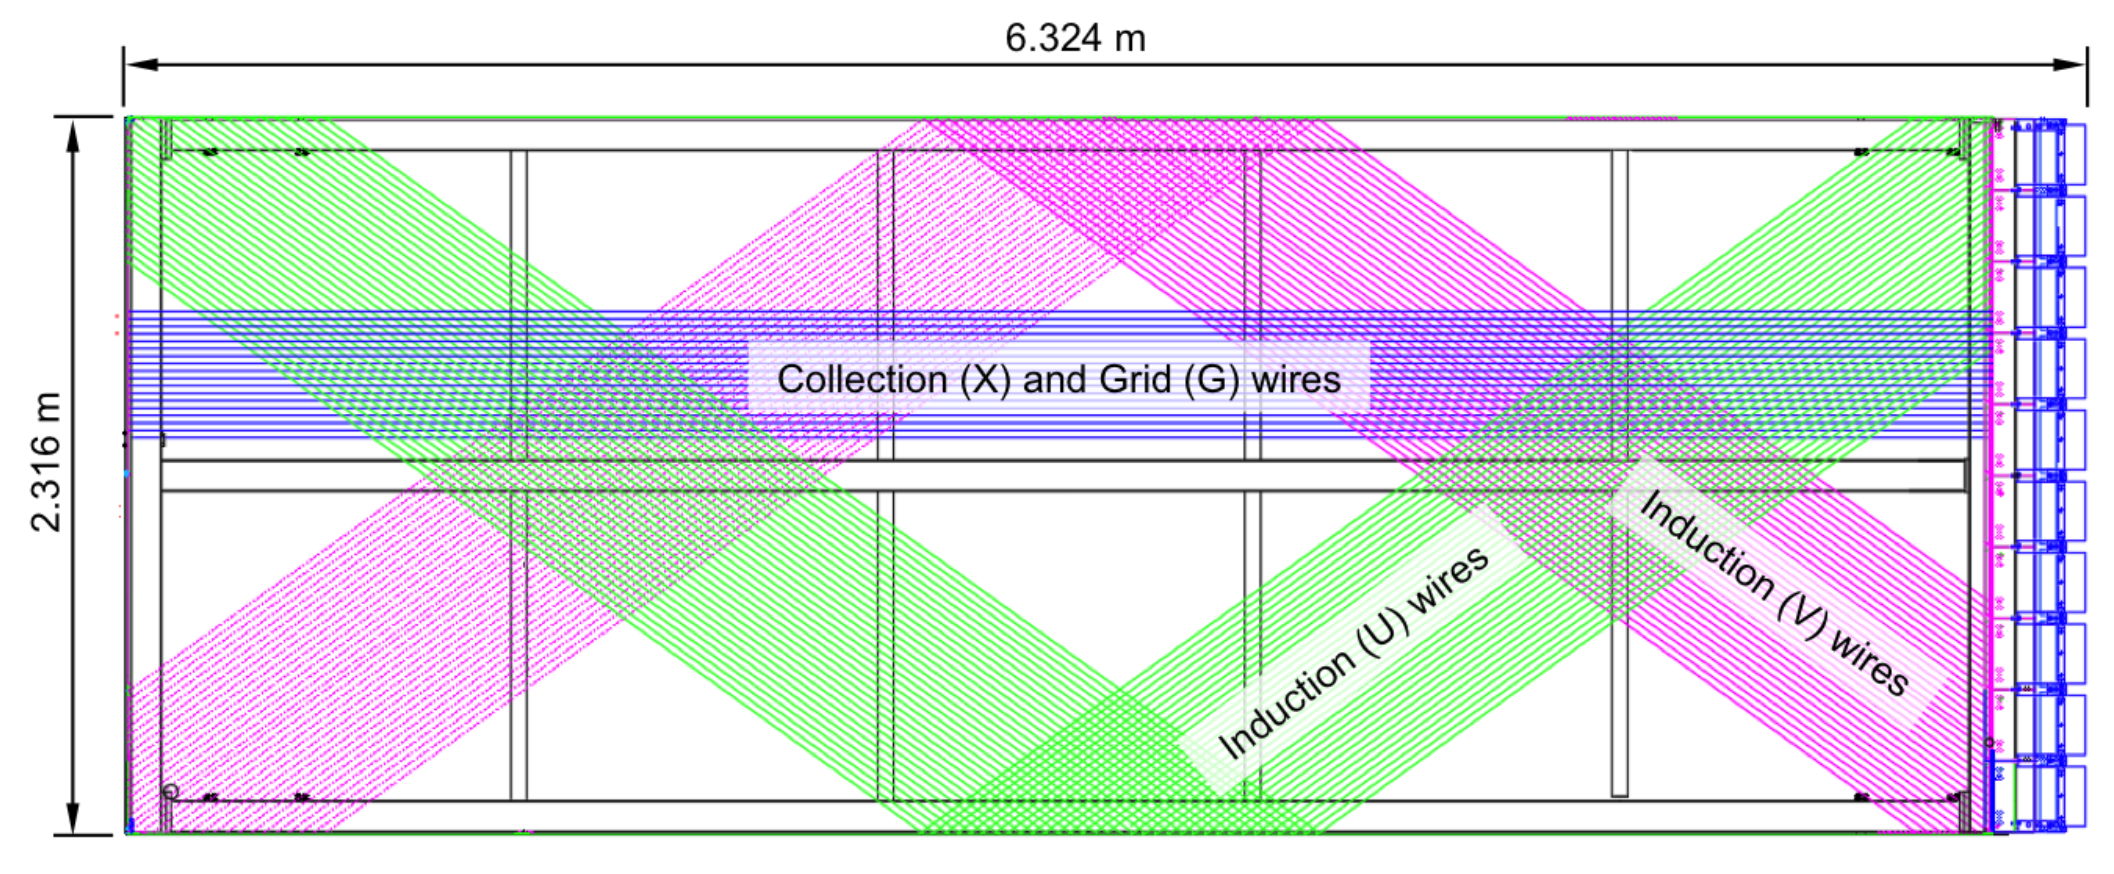
\includegraphics[width=1\linewidth]{Images/DUNE/FD/APA_wires}
	\caption[Schematic representation of an APA frames showing the U, V, X and G wires.]{Schematic representation of an APA. The black lines represent the APA steel frame. The green and magenta lines correspond to the direction of the U and V induction wires respectively. The blue lines indicate the direction of the X collection wires and the wire shielding G. Figure taken from Ref. \cite{DUNE2020TDR1}.}
	\label{fig:apa}
\end{figure}

The front-end readout electronics, or cold electronics as they are immerse in the LAr, are attached to the top of the up APAs and the bottom of the down APAs. Mounted on the front-end mother boards we have a series of ASICs that digitize the signals from the collection and induction planes. Each wire signal goes to a charge-sensitive amplifier, then there is a pulse-shaping circuit and this is followed by the analogue-to-digital converter. This part of the process happens inside the LAr to minimise the number of cables penetrating the cryostat. The digitised signals come out finally via a series of high-speed serial links to the warm interface boards (WIBs), from where the data is sent to the back-end DAQ through optical fibers.

\begin{figure}[h!]
	\begin{subfigure}{0.49\textwidth}
		\centering
		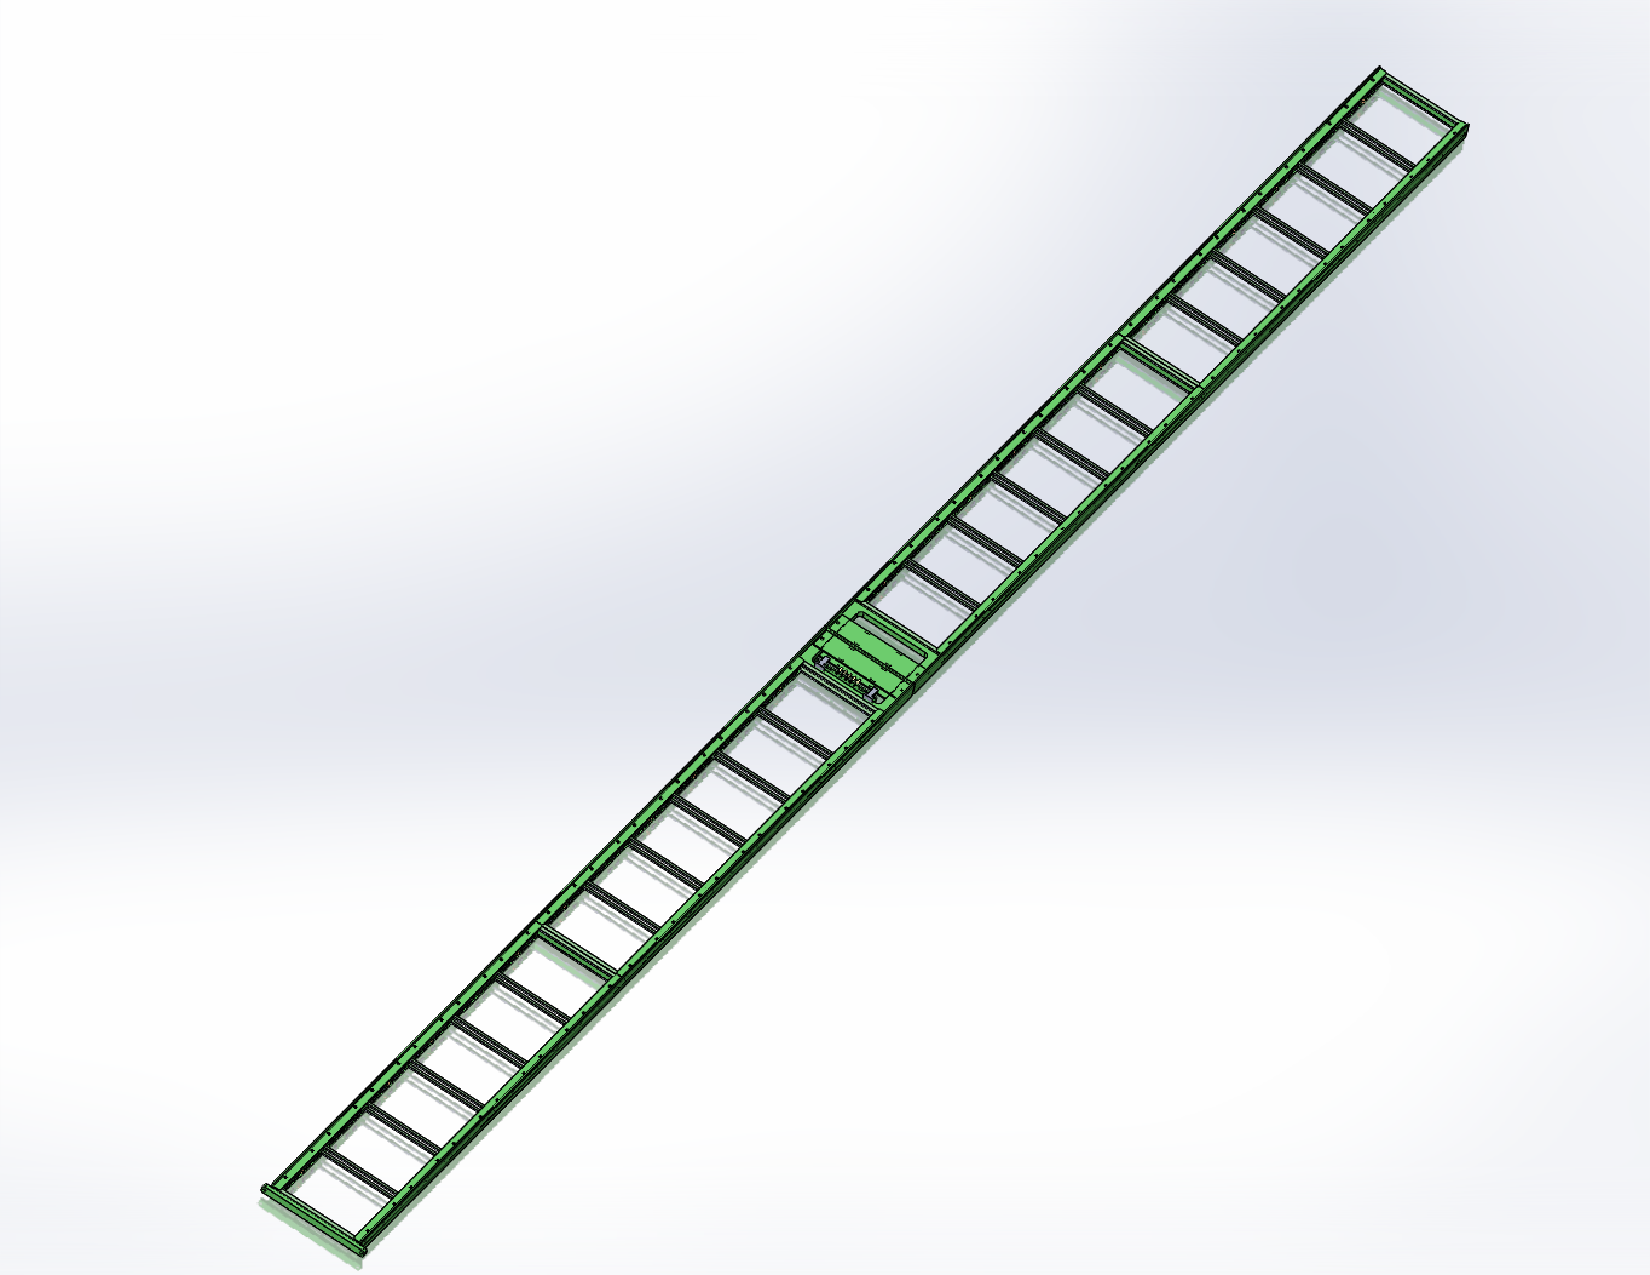
\includegraphics[width=.90\linewidth]{Images/DUNE/FD/pds-module}
	\end{subfigure}
	\begin{subfigure}{0.49\textwidth}
		\centering
		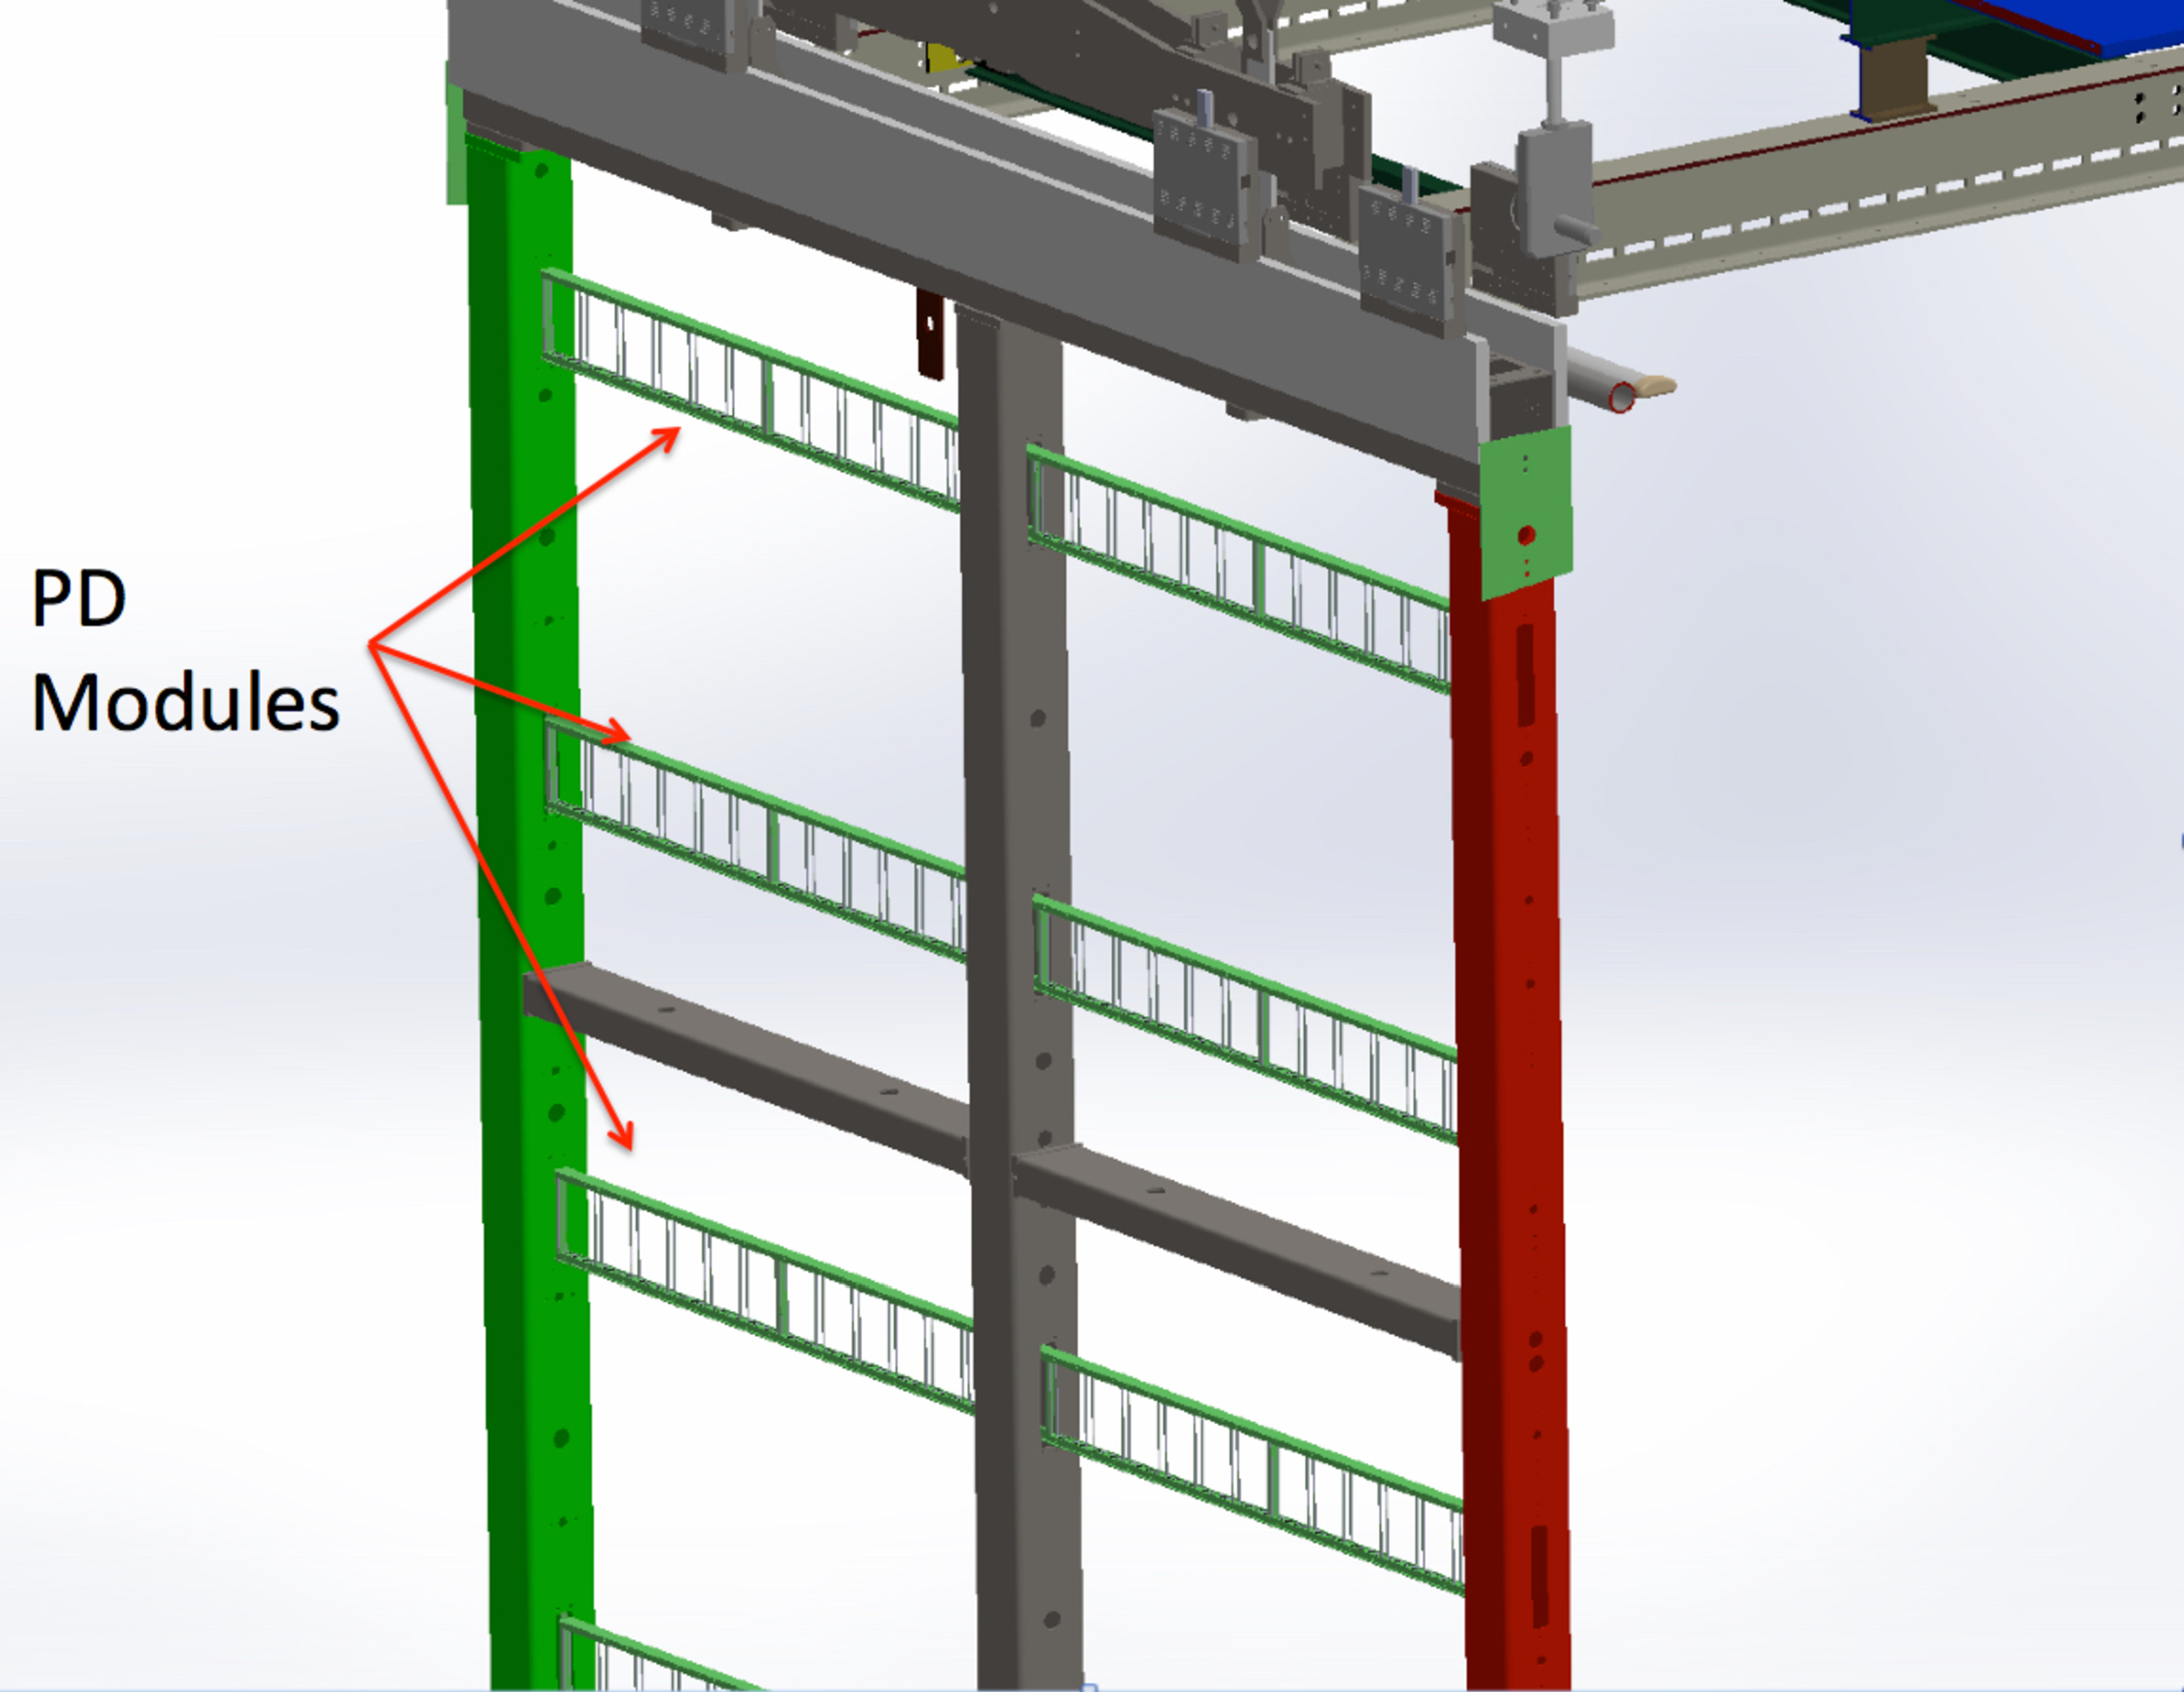
\includegraphics[width=.90\linewidth]{Images/DUNE/FD/pds-in-apa-assembly}
	\end{subfigure}
	\caption[A PDS module containing 24 X-ARAPUCAs and the location of the modules on the APAs.]{A PDS module containing 24 X-ARAPUCAs (left) and the location of the modules on the APAs (right). Figure taken from Ref. \cite{DUNE2020TDR1}.}
	\label{fig:dune_pds}
\end{figure}

The PDS uses modules of X-ARAPUCA devices, mounted on the APA frames between the wire planes. Each X-ARAPUCA consists of layers of dichroic filter and wavelength-shifter. They shift the VUV scintillation light into the visible spectrum, sending then the visible photons to silicon photomultiplier (SiPM) devices. The PDS modules are $209~\mathrm{cm}\times12~\mathrm{cm}\times2~\mathrm{cm}$ bars, containing 24 X-ARAPUCAs. There are 10 of these PDS modules per APA. Fig. \ref{fig:dune_pds} shows a PDS module (left) and the placement of the modules on the APAs (right).

\begin{comment}
	When using a SP LArTPC there is no electron amplification, thus low noise is required by CE to extract the signals from the wires with a minimum S/N. In the worst operating case (short drift electron lifetime $\tau = 3 \ \mathrm{ms}$ and $E_{drift} = 250 \ \mathrm{V/cm}$) at least $10^{4}$ electrons will arrive to the anode from a minimum ionizing particle (MIP) near the cathode (farthest possible distance). Requiring at most $10^{3}$ electrons of equivalent noise charge (ENC) we will have a S/N $~\sim10$ for the collection wires. In the induction wires it results in S/N $\sim 5$, because of the bipolar shape of the signal. Keeping noise low (improving S/N) is crucial to achieve the physics goals. It allows proper event reconstruction and expand the boundaries on low-energy phenomena (SNB, $^{39}$Ar calibrations, etc.). Noise also affect DAQ bandwidth, and can be a problem for astrophysical measurements.
\end{comment}

\subsection{Vertical Drift}

\begin{figure}[t]
	\centering
	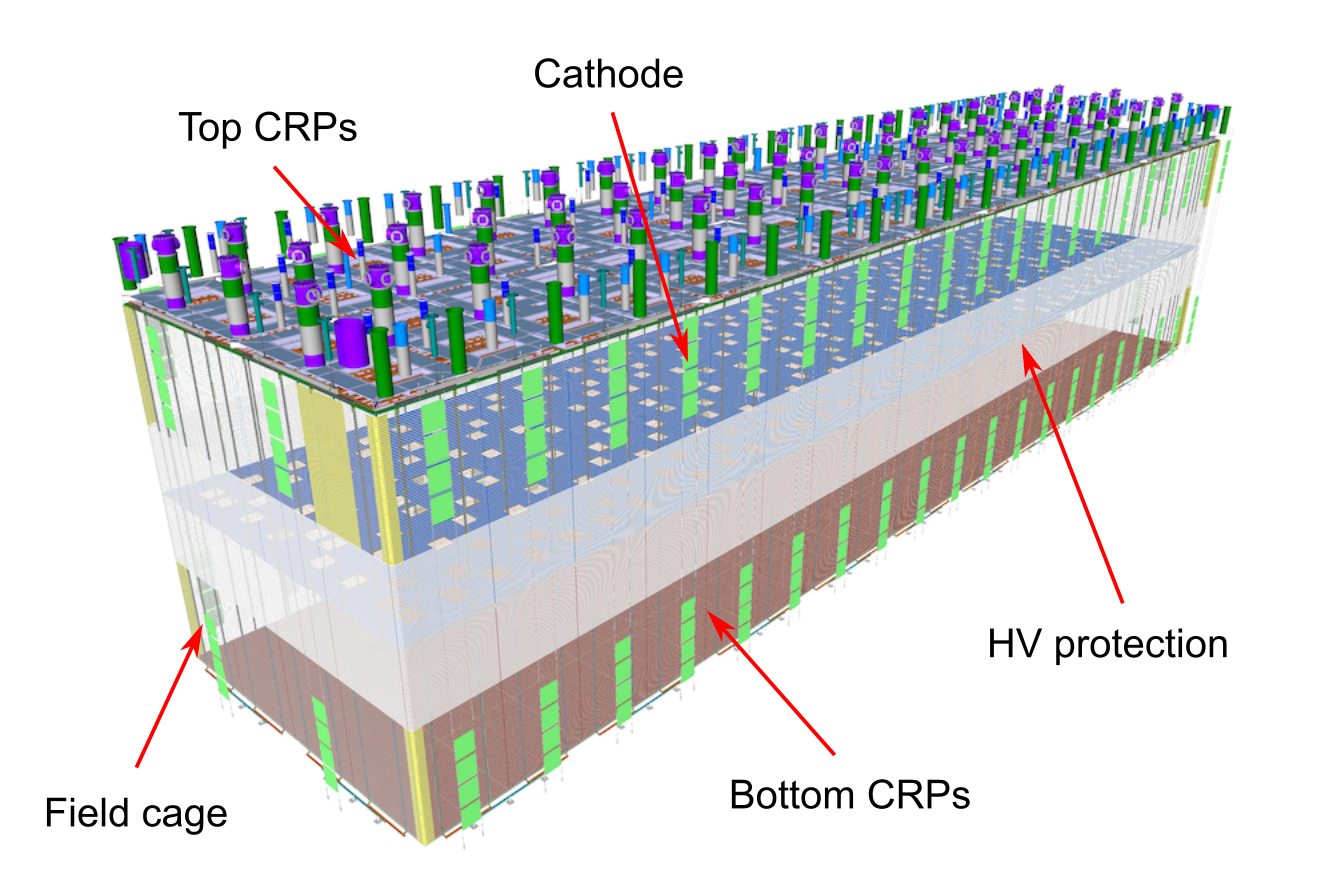
\includegraphics[width=0.70\linewidth]{Images/DUNE/FD/dune_vd}
	\caption[Proposed design for the FD-3 module following the VD principle.]{Proposed design for the FD-3 module following the VD principle. Figure adapted from Ref. \cite{DUNEVDTDR}.}
	\label{fig:dune_vd}
\end{figure}

In the VD case the ionisation electrons will drift vertically until they meet a printed circuit board-based (PCB) readout plane. It is based on the original dual-phase (DP) design deployed at CERN, known as ProtoDUNE-DP, used a vertical drift design with an additional amplification of the ionization electrons using a gaseous argon (GAr) layer above the liquid phase. The VD module incorporates the positive features of the DP design without the complications of having the LAr-GAr interface.

The current design of the FD VD module counts with two drift chambers with a maximum drift distance of $6.5~\mathrm{cm}$. A cathode plane splits the detector volume along the drift direction while the two anode planes are connected to the bottom and top walls of the detector. The layout of the VD module is shown in Fig. \ref{fig:dune_vd}. Compared with the HD design, the VD option offers a slightly larger instrumented volume and a more cost-effective solution for the charge readout.

\begin{figure}[t]
	\centering
	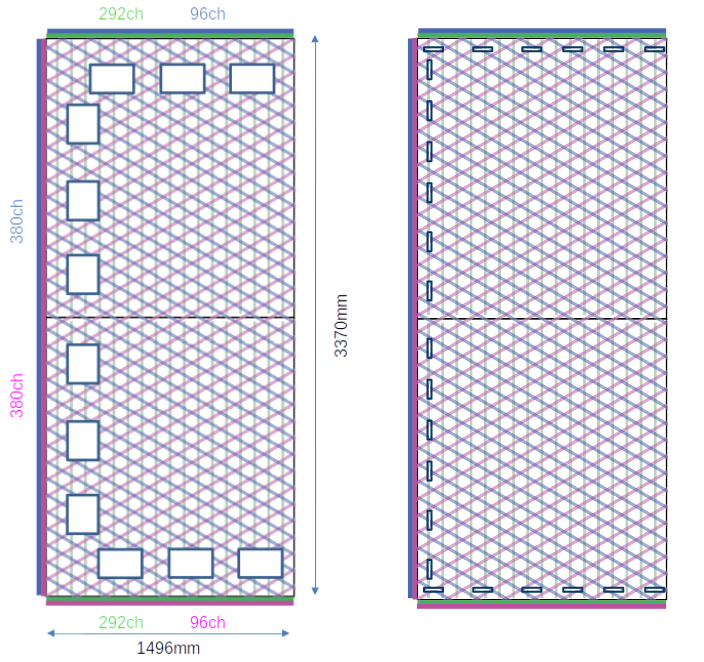
\includegraphics[width=0.70\linewidth]{Images/DUNE/FD/3V_anode_layout}
	\caption[Schematic representation of the electrode strip configuration for a top and bottom CRU.]{Schematic representation of the electrode strip configuration for a top (left) and bottom (right) CRU. Figure taken from Ref. \cite{DUNEVDTDR}.}
	\label{fig:dune_cru}
\end{figure}

As in the HD design, each drift volume features a $500~\mathrm{V/cm}$ electric field and a field cage that ensures its uniformity. The anode planes are arrays of $3.4~\mathrm{m}\times3~\mathrm{m}$ charge-readout planes (CRPs). These are formed by a pair of charge-readout units (CRUs), which are built from two double-sided perforated PCBs, with their perforations aligned. The perforations allow the drift electrons to pass between the layers.

The PCB face opposite to the cathode has a copper guard plane which acts as shielding, while its reverse face is etched with electrode strips forming the first induction plane. The outer PCB has electrode strips on both faces, the ones facing the inner PCB form the second induction plane while the outermost ones form the collection plane. Fig. \ref{fig:dune_cru} shows the layout of the electrode strips for the top (left) and bottom (right) CRUs. The magenta and blue lines represent the first and second induction planes respectively, and the green lines correspond to the collection plane.

The PDS in the VD module will use the same X-ARAPUCA technology developed for the HD design. The plan is to place the PDS modules on the cryostat walls and on the cathode, in order to maximise the photon yield.

%\subsection{Module of opportunity}

\begin{figure}[t]
	\centering
	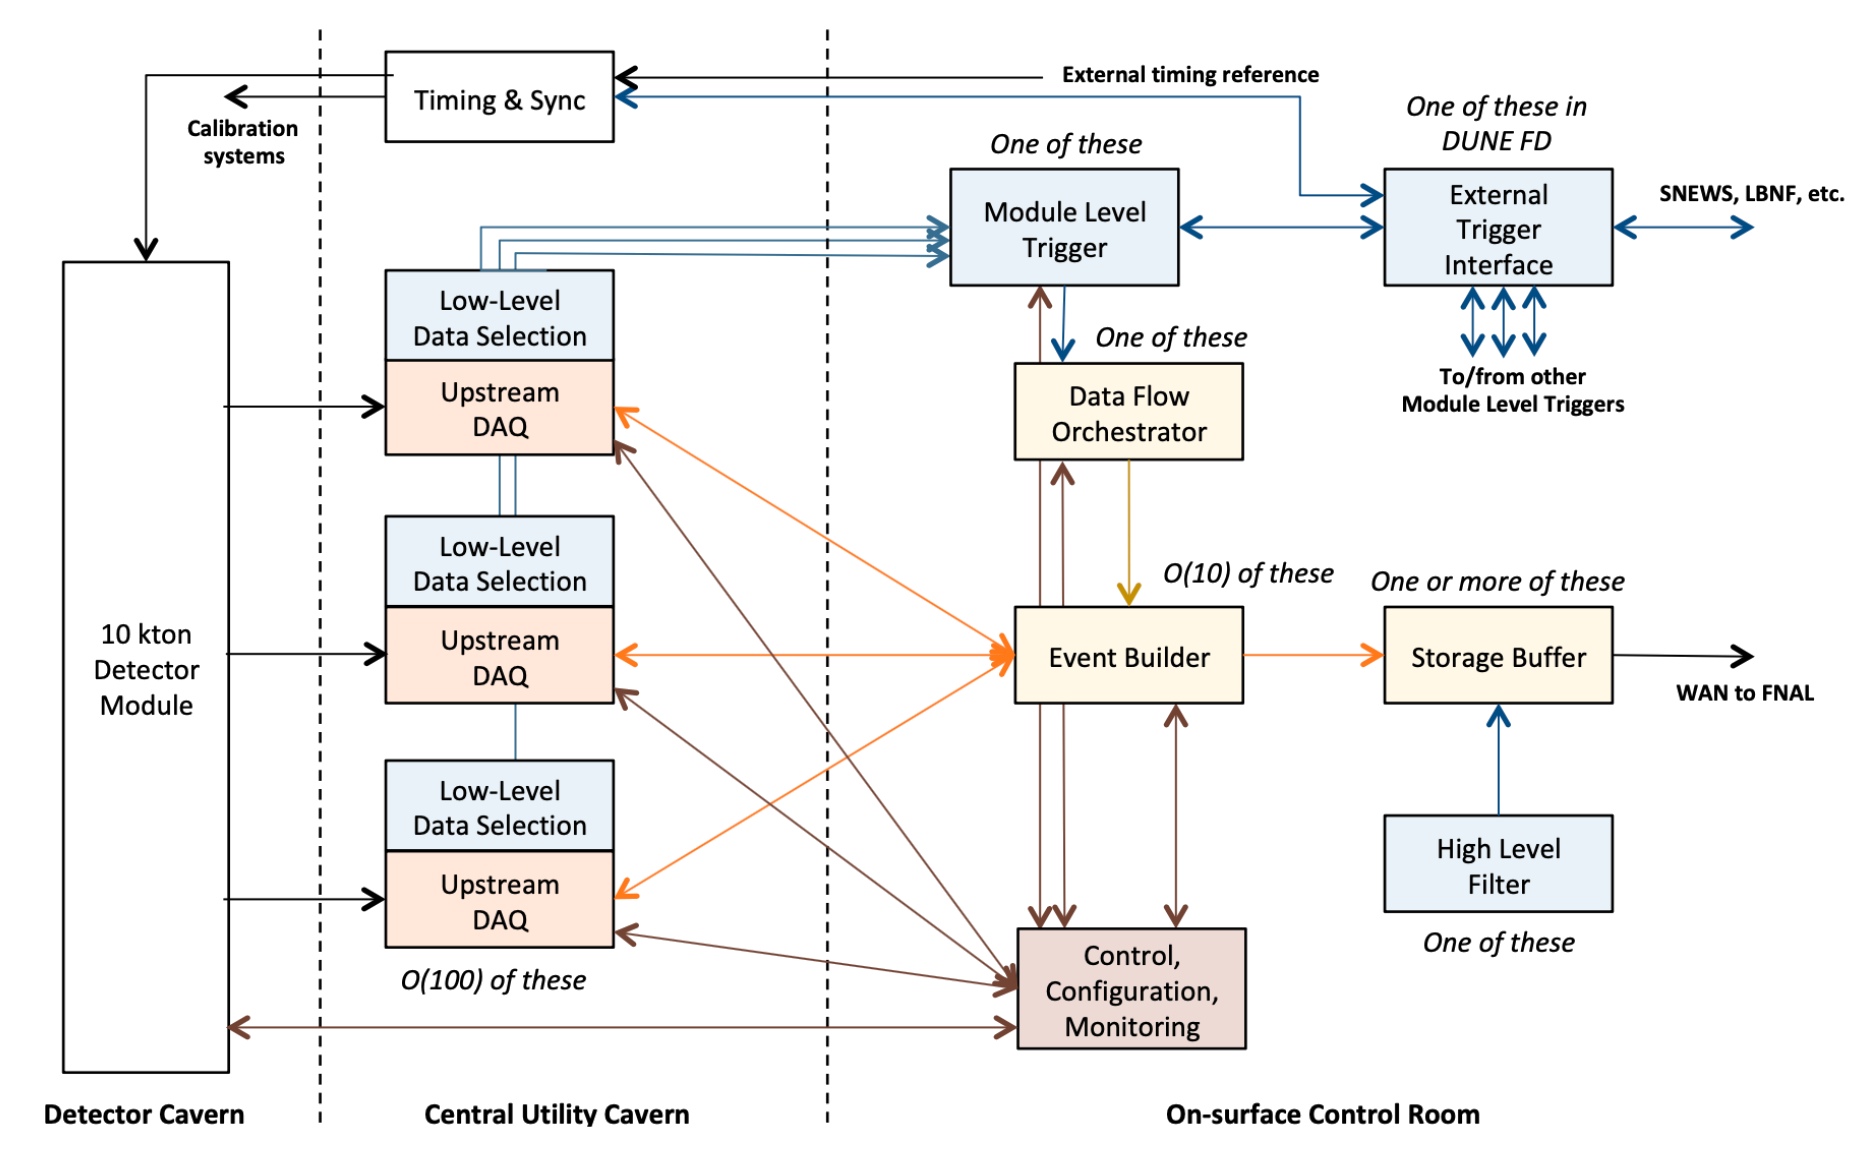
\includegraphics[width=0.8\linewidth]{Images/DUNE/FD/DAQ_detailed2}
	\caption[Detailed diagram of the DUNE FD DAQ system.]{Detailed diagram of the DUNE FD DAQ system. Figure taken from Ref. \cite{DUNE2020TDR4}.}
	\label{fig:daq1}
\end{figure}

\subsection{FD Data Acquisition System}

The data acquisition (DAQ) system receives, processes and stores data from the detector modules. In the case of DUNE the DAQ architecture is designed to work for all FD modules interchangeably, except some aspects of the upstream part which may depend on the specific module technology.

The enormous sample rate and the number of channels in TPC and PD readouts will produce a very large volume of data. These pose really strong requirements and challenges to the DUNE FD DAQ architecture. It will be required to read out data of the order of ten thousand or more channels at rates of a few MHz. To cope with the huge data volume, segmented readouts and compression algorithms are used to reduce the data rate to manageable levels.

The DAQ system of the DUNE FD is composed of five different subsystems. The first one is the upstream DAQ, which receives the raw data from the detector, buffers it and perform some low-level pre-processing. The minimally processed data is then fed into a hierarchical data selection system, which then performs a module level trigger decision. In case of a positive decision a trigger command is produced and executed by the data flow orchestrator, located in the back-end (BE) DAQ subsystem. Subsequently the DAQ BE retrieves the relevant data from the buffers located in the upstream DAQ, adds all the data into a cohesive record and saves it to permanent storage. Watching over all the other subsystems we also have the control, configuration and monitoring subsystem and the time and synchronization subsystem. Figure \ref{fig:daq1} shows a schematic diagram of the DAQ system, showing the different subsystems and their relations.

A notorious challenge for the DUNE DAQ system comes from its broad physics goals. We must be prepared to process events spanning a wide range of time windows (from $5 \ \mathrm{ms}$ in the case of beam and cosmic neutrinos and nucleon decay to $100 \ \mathrm{s}$ in the case of SNBs) and therefore this requires a continuous readout of the detector modules. Moreover, because of the off-beam measurements we need to ensure the capabilities of online data processing and self-triggering. Having this into account, together with the technical constraints, the DUNE FD DAQ faces a series of challenges: it needs to be fault tolerant and redundant to reduce downtime, accommodate new components while it keeps serving the operational modules, have large upstream buffers to handle SNB physics, be able to support a wide range of readout windows and last reduce the throughput of data to permanent storage to be at most $30 \ \mathrm{PB/year}$.